\documentclass[a4paper,11pt]{report}

\usepackage[utf8x]{inputenc}
\usepackage[italian]{babel}
%\usepackage[babel]{csquotes}
%\usepackage[style=alphabetic,indexing]{biblatex}
\usepackage[space]{cite}

\usepackage{listings}
\usepackage[cc]{titlepic}
\usepackage {graphicx}
\usepackage {url}
\usepackage{lscape}



\lstloadlanguages{[ANSI]C}

\title{\vspace*{-3cm}{\includegraphics[width=90mm]{torVergataLogo.jpg}\\ \vspace{.5cm}
       % \vspace{1cm}
        \textbf{UNIVERSIT\`A DEGLI STUDI DI ROMA\\TOR VERGATA\\} \vspace{1cm}
       %\Large{FACOLT\`A DI INGEGNERIA} \\ \vspace{1.5cm}
       \Large{CORSO DI LAUREA IN\\ INGEGNERIA INFORMATICA}\\ \vspace{.5cm}
       \large{A.A.  2010-2011 \vspace{.5cm}\\\textbf{Tesi di Laurea}}\\ \vspace{.5cm}
       \LARGE{\textbf{At First Look in Map Reduce}\\}
       \LARGE{Ricerca in streaming di componenti connesse e biconnesse di grafi tramite cluster}\\
       }}

%\title{\textbf{At First Look in Map Reduce}\\Ricerca in streaming di componenti connesse e biconnesse di grafi tramite cluster}
\author{\vspace{1cm}\\
\begin{tabular}{c c}
\hspace{-2cm}\LARGE{Emanuele Paracone} &\hspace{3cm} 
\begin{tabular}{c c}
 \LARGE{ \textbf{Relatori:}} &\LARGE{Prof. Luigi Laura}\\
      &\LARGE{Prof. Giuseppe Italiano}\\
\end{tabular}
\end{tabular}
\vspace{2cm}
 } 

\date{\Large{19 Luglio 2011}}
%\titlepic{\includegraphics[width=\textwidth]{torVergataLogo.jpg}}




\begin{document}



\maketitle

\tableofcontents

\chapter*{}
\vspace{12cm}
\hspace{9cm}\includegraphics[width=37mm]{images/k&t.png}


\chapter*{Compendio}
In questo lavoro di tesi analizziamo una soluzione al problema della ricerca esaustiva, in un grafo, delle componenti connesse, delle
componenti biconnesse, degli \emph{articulation points}
 e dei \emph{bridges},
ottenuta elaborando uno stream in input in modo parallelo secondo il paradigma MapReduce.
\paragraph{} Descriviamo l'algoritmo At First Look, il paradigma
 MapReduce e la sua implementazione nel framework Apache Hadoop, analizzando poi i programmi \emph{Hitsura}, la nostra implementazione di At
First Look, e \emph{HitSoop}, l'oggetto della nostra tesi, 
che implementa una soluzione al problema secondo il paradigma MapReduce.

\chapter*{Introduzione}
L'oggetto di questo lavoro di tesi è la nostra soluzione al problema della ricerca esaustiva delle componenti connesse, delle componenti
biconnesse, degli \emph{articulation points}
 e dei \emph{bridges} di un grafo in input descritto da uno \emph{stream} di dimensioni molto maggiori della disponibilità di memoria media
di una singola macchina. \emph{Autonomous Systems},
generiche reti di calcolatori, e molti altri sono gli scenari nei quali è interessante estrarre dette informazioni dai grafi che li
modellano. Abbiamo 
implementato perciò il programma HitSoop, che raggiunge lo scopo distribuendo il lavoro complessivo su un cluster di elaboratori secondo il
paradigma MapReduce.
HitSoop è un programma scritto in Java per Apache Hadoop, il framework della Apache Foundation che implementa il paradigma MapReduce,
eseguito
su un cluster Amazon Web Services EC2.
\paragraph{}
Nell'implementazione di HitSoop ci siamo ispirati all'algoritmo At First Look, che affronta lo stesso problema secondo il modello del
\emph{classical streaming},
ed abbiamo costruito un nuovo algoritmo in grado di processare lo stream in input in modo non sequenziale, attraverso l'aggregazione delle
elaborazioni intermedie effettuate su porzioni
distinte dell'input complessivo. 
\paragraph{}
L'interesse per l'implementazione MapReduce proviene dal sensibile vataggio in termini prestazionali che è possibile ottenere
parallelizzando quanto più possibile
il lavoro complessivo. Il calcolo parallelo ed il cloud, infatti, sono sempre più al centro delle attenzioni di aziende di IT di qualunque
dimensione, in quanto permettono
un deciso abbattimento dei costi. 

\chapter{At First Look}\label{At First Look}
\section{Cos'è ``At First Look'' }
\paragraph{}
\emph{\textbf{At First Look}} (AFL) è un algoritmo che analizza la topologia di un grafo generico non diretto e ricerca esaustivamente
all'interno di questo:
\begin{itemize}
 \item le componenti connesse (\textbf{CC});
 \item le componenti bi-connesse(\textbf{BCC});
 \item gli articulation points;
 \item i bridges.
\end{itemize}
\par
Queste informazioni sono utili in scenari reali per l'analisi delle proprietà strutturali di grafi che modellano reti esistenti
dimensionalmente complesse,
come quelle degli indirizzi di un \emph{Autonomous System} (AS) o delle relazioni astratte tipiche dei casi di studio di vari contesti
(ricerca scentifica, Social Engineering, ecc.),
e la loro ricerca off-line è un problema che risale agli anni settanta.
\paragraph{}
At First Look ottiene queste informazioni on-line, ovvero processando sequenzialmente il data-streaming che descrive gli archi del grafo che
si vuole analizzare, attenendosi  
ai vincoli del \emph{classical streaming} sul tempo di processamento delle informazioni (\textbf{PIPT} - Per Item Processing Time) e sullo
spazio di memoria occupato.
\paragraph{}
\centerline{\includegraphics[width=100mm]{images/grafo_input_notit.png}} 
\paragraph{}
In questo capitolo tratteremo il modello del classical streaming e dei vincoli che ne derivano sulla disponibilità di memoria e sul
\emph{PIPT} rispetto alla
dimensione dello stream in input, la struttura e le caratteristiche del grafo a foresta \emph{Navigational Sketch} in cui vengono
progressivamente modellate 
le informazioni sulla topologia del grafo in input, il funzionamento dell'algoritmo At First Look, la dimostrazione della sua correttezza
durante l'esecuzione,
la gestione della memoria e la struttura dati del Navigational Sketch, ed infine l'analisi delle prestazioni e del costo dell'algoritmo.
\subsection{Componenti Connesse (\textbf{CC})}
Una componente connessa $CC$ di un grafo non orientato \textbf{G}(V,E) con $V$ nodi e $E$ archi è un insieme di nodi $n_i \in V $ tali che
\\\\
\centerline{$n_i \in CC_j \Longrightarrow
 \forall n_j \in CC \wedge n_j \neq n_i \ $}\\\centerline{$ \exists\  percorso(n_i,n_j) = \{
 arco\left(n_i,n_1\right),arco\left(n_1,n_2\right),...,arco\left(n_{n-1},n_j\right) \}.$}
\\\\
cioè per ogni nodo appartenente ad una componente connessa $CC_i$ esiste almeno un percorso verso ogni altro nodo 
appartenente alla stessa componente connessa, e nessun percorso verso alcun altro nodo.
\\\\
\centerline{\includegraphics[width=100mm]{images/componenti_connesse_notit.png}} 
\subsection{Componenti Bi-Connesse (\textbf{BCC})}\label{Componenti Bi-Connesse}
Una componente bi-connessa $BCC$ in un grafo non orientato \textbf{G}(V,E) è un insieme di nodi $n_i \in V $ tali che \\\\
\centerline{$n_i \in BCC \Longrightarrow \forall n_j \in BCC \wedge n_j \neq n_i $}\\\centerline{$ \exists\ \# > 1\ di\ percorsi(n_i,n_j)
.$}
\\\\
ovvero presi due nodi $u,v\in BCC$ esistono almeno due percorsi distinti tra $u$ e $v$ in \textbf{G}.\\\\
\centerline{\includegraphics[width=100mm]{images/componenti_biconnesse_notit.png}}
\subsection{Articulation Points}
Un \emph{articulation point} è un vertice $v\in V$ tale che la sua rimozione da \textbf{G} aumenta il numero di componenti connesse in
\textbf{G}.\\\\
\centerline{\includegraphics[width=100mm]{images/articulation_point_notit.png}}

\subsection{Bridges}
Un \emph{bridge} è un arco $e \in E$ tale che la sua rimozione da \textbf{G} aumenta il numero di componenti connesse in \textbf{G}.\\\\
\centerline{\includegraphics[width=100mm]{images/bridges_notit.png}}


\section{Il \emph{classical streaming}}
Nel \emph{classical streaming} l'input è un data-stream che viene letto in modo sequenziale e che deve essere processato con una
disponibilità di memoria
molto minore rispetto alla dimensione dello stream.\\
Com'è facile intuire i problemi connessi riguardano: 
\begin{itemize}
 \item la velocità con cui ogni informazione prelevata dallo stream viene processata (\textbf{PIPT}) rispetto alla lunghezza di questo;
 \item il calcolo dell'output mantenendo una quantità di informazioni minore rispetto a quella dell'input.
\end{itemize}
\subsection{Per Item Processing Time}
Più avanti nel capitolo proveremo che il tempo $T$ speso da At First Look per processare l'intero input di un grafo con $n$ nodi e $m$ archi
verifica
$T \in O \left(n\* \log\left(n\right) + m\alpha\left(m,n\right)\right)$ (dove $\alpha$ è l'inverso della funzione di Ackermann),  da cui
otteniamo il tempo medio $T_i$ di processamento per 
record dello stream:\\\\
\centerline{$T_i \in O\left( \log \left( n\right)+{m\over{n}}\alpha\left(m,n \right) \right)$}
\subsection{Limitazioni di memoria}
Tipicamente lo stream in input ha una dimensione molto maggiore della quantità di memoria disponibile per la computazione. Siccome lo stream
viene processato 
sequenzialmente record per record, l'output finale deve essere ottenuto modificando progressivamente una struttura dati che sintetizzi
correttamente tutte e sole
le informazioni strettamente necessarie.
\paragraph{} 
L'informazione complessiva dell'input viene ``compressa'' all'interno della struttura dati, di cui viene modificato lo stato fino al
raggiungimento di
 uno stato finale quando viene consumato l'intero streaming.
\subsection{Algoritmi e streaming}
La classe di problemi che possono essere affrontati con un modello streaming è composta da quei problemi che ammettono soluzioni che
rispettino i vincoli
sul PIPT e sulla richiesta di memoria appena descritti. \par
La ricerca di \emph{connected components} è un problema noto appartenente alla classe appena descritta.

\section{Navigational Sketch}
\emph{At First Look} sfrutta una struttura dati detta \emph{\textbf{Navigational Sketch}} che modella la topologia di un grafo relativamente
a componenti connesse e biconnesse, 
\emph{articulation points} e \emph{edges}.
\paragraph{}
\centerline{\includegraphics[width=120mm]{images/da_grafo_a_NS.png}}
\subsection{La struttura di un Navigational Sketch}
\paragraph{}
Il \emph{Navigational Sketch} \emph{\textbf{NS}} di un grafo generico \mbox{$G=(V,E)$} è una foresta \mbox{$NS=(V_{ns},E_{ns})$} in cui
l'insieme di nodi $V_{ns}$ è lo stesso
 di $G$ (ovvero\mbox{ $V_{ns}=V$}),
mentre l'insieme degli archi $E_{ns}$ è composto da archi \emph{solid} e archi \emph{colored}.
\paragraph{}\paragraph{}
\centerline{\includegraphics[width=130mm]{images/navigational-sketch_notit.png}}
\paragraph{}
Un \emph{Navigational Sketch} \emph{NS} ha le seguenti proprietà:
\begin{enumerate}
 \item gli alberi in \emph{NS} modellano le componenti connesse di $G$;
 \item gli archi \emph{solid} in NS sono i \emph{bridges} di $G$;
 \item le componenti biconnesse di $G$ sono rappresentate da sottoalberi in \emph{NS} formati:
\begin{itemize}
 \item da un nodo padre e $b-1$ nodi figli (dove $b$ è il numero di nodi appartenenti alla 
stessa componente biconnessa);
 \item da archi tutti di uno stesso colore, unico in \emph{NS}.
\end{itemize}
\end{enumerate}



\subsection{\emph{Color degree} di un nodo nel Navigational Sketch} \label{Color degree di un nodo nel Navigational Sketch}
Il \emph{\textbf{color degree}} di un nodo $i$ di \emph{NS} ($d_c(i)$) corrisponde alla somma del numero di archi \emph{solid} incidenti su
$i$ più il numero
di diversi colori degli archi incidenti su $i$.
\paragraph{}
Ad esempio un nodo $i$ con dieci archi di uno stesso colore e due archi \emph{solid} avrà grado \\\centerline{$d_c(i)=1+2=3$,}\\\\ mentre un
nodo $j$ con dieci archi \emph{solid} e due \emph{colored} di colori
diversi avrà grado \\\centerline{$d_c(j)=10+2=12$.}
\paragraph{Lemma:}
Un nodo $n$ il cui grado $d_c(n)$ sia maggiore di 1 è un \emph{articulation point} di $G$. 
\paragraph{Dimostrazione:}Un nodo siffatto infatti verifica almeno una delle proprietà:
\begin{itemize}
 \item $n$ appartiene a più di una comopnente biconnessa;
 \item $n$ appartiene ad una componente biconnessa ed è adiacente ad almeno un \emph{bridge};
 \item $n$ è adiacente a più di un \emph{bridge}.
\end{itemize}

\section{L'algoritmo At First Look}
\subsection{Definizione del problema}
Il problema su cui At First Look opera è il seguente:
\\
preso un grafo generico $G$ rappresentato come stream possibilmente non ordinato dei suoi archi, si vogliono calcolare in modo esaustivo le
proprietà di connettività:
\begin{itemize}
 \item componenti connesse;
 \item componenti biconnesse;
 \item \emph{articulation points};
 \item \emph{bridges}.
\end{itemize}

\subsection{Processamento dello stream}
At First Look consuma lo stream in input arco per arco fino al suo esaurimento e ottiene l'output definitivo modificando nel corso
dell'elaborazione lo stato di un
\emph{Navigational Sketch \textbf{NS}} mantenuto in memoria. Una volta terminata la lettura dell'input, il \emph{NS} conterrà tutte le
informazioni riguardanti 
componenti connesse e biconnesse, \emph{articulation points} e \emph{bridges} del grafo $G$ descritto nello stream di input.
\paragraph{}
Le operazioni necessarie all'aggiornamento del \emph{NS} sono: 
\begin{enumerate}
 \item verifica quando due nodi sono nello stesso albero della foresta;
 \item unione di alberi;
 \item verifica quando due nodi sono estremi degli stessi archi colorati;
 \item trova il percorso che collega due nodi.
\end{enumerate}
Queste operazioni vengono compiute in funzione dell'azione richiesta per l'ultimo arco correntemente letto dallo stream.
\subsection{Come funziona At First Look}\label{Come funziona At First Look}
At First Look processa gli archi in input nel seguente modo:
\begin{enumerate}
 \item se l'arco corrente unisce due alberi distinti allora verrà aggiunto come arco \emph{solid}. Infatti sarebbe l'unico arco che collega
due componenti di connesse e quindi un 
\emph{bridge} per definizione;
 \item se l'arco corrente connette due nodi $u,v$ all'interno della stessa componente connessa distinguiamo due casi relativamente al tipo
di archi nel percorso tra $u$ e $v$:
 \begin{enumerate}
  \item tutti gli archi nel percorso da $u$ a $v$ \textbf{sono dello stesso colore}: in questo caso $u$ e $v$ sono già nella stessa
componente biconnessa;
  \item il percorso tra $u$ e $v$ è composto da archi di \textbf{tipo e/o colore diverso}: in questo caso, esiste un nuovo percorso per
ognuno dei nodi coinvolti e deve 
essere costruita un'opportuna componente biconnessa cui questi appartengono. \\Tutte le componenti biconnesse ``toccate'' dal percorso
devono essere unite in una unica, tramite i passi:
  \begin{enumerate}
   \item costruzione del set $N$ di tutti i nodi coinvolti, ovvero tutti i nodi per i quali passa il percorso da $u$ a $v$ e tutti i nodi
appartenenti alle componenti biconnesse
attraversate dal percorso;
   \item rimozione di tutti gli archi incidenti ad ogni nodo $n \in N$;
   \item scelta di un nodo $n_f \in N$ che diverrà il nodo ``\emph{nodo padre}'' del sottoalbero rappresentante la nuova componente
biconnessa;
   \item aggiunta di un arco \emph{colored} dello stesso colore tra $n_f$ ed ognuno dei nodi figli $n_i \in N$ con $n_i \neq n_f$.
  \end{enumerate}
 \end{enumerate}
\end{enumerate}
\paragraph{}
\centerline{\includegraphics[width=150mm]{images/modifiche_ns.png}} 
\section{Correttezza di At First Look}\label{Correttezza di At First Look}
\subsection{Invarianti}
Per dimostrare la correttezza dell'algoritmo dobbiamo dimostrare che ad ogni passo dell'elaborazione, ovvero per ogni processamento di
un arco letto dallo stream in input, valgano i seguenti invarianti:
\begin{enumerate}
 \item ad ogni passo un albero nel \emph{Navigational Sketch} è una componente connessa;
 \item ad ogni passo un nodo adiacente ad un arco di colore $c$ appartiene alla componente biconnessa rappresentata da $c$;
 \item ad ogni passo ogni arco \emph{solid} è un \emph{bridge};
 \item ad ogni passo ogni nodo $n$ tale che $d_c(n) > 1$ è un \emph{articulation point}.
\end{enumerate}

\subsection{Alberi e componenti connesse}\label{Alberi e componenti connesse}
\paragraph{Teorema 1:}\emph{ad ogni passo un albero nel Navigational Sketch è una componente connessa.}
\paragraph{Dimostrazione:} dimostriamo la correttezza del teorema per induzione sulla lunghezza dello stream di archi in input letto.
\paragraph{}
Nel \emph{caso base} non sono ancora stati letti archi dallo stream, il \emph{Navigational Sketch NS} è privo di archi e ogni suo nodo è un
albero singleton.
È facile osservare la correttezza del teorema per \emph{NS}, in quanto, non essendoci archi tra i nodi, ogni nodo è l'unico elemento di una
componente connessa.
\paragraph{}
Assumendo che sia stata dimostrata la correttezza del teorema al passo $k$, cioè dopo aver prelevato dallo stream $k$ archi, vogliamo
dimostrare che questa vale anche al passo $n+1$. 
Aggiungendo un nuovo arco $e$ a \emph{NS} si può verificare che:
\begin{itemize}
 \item $e$ collega due nodi appartenenti ad alberi differenti in \emph{NS}. In questo caso AFL unisce i due alberi in uno unico. Il teorema
vale ancora dopo l'aggiunta di $e$
in quanto i due alberi uniti sono due componenti connesse che all'aggiunta di $e$ vengono collegate tra loro divenendo un'unica CC.
 \item $e$ collega due nodi appartenenti allo stesso albero in \emph{NS}. In questo caso le eventuali modifiche di \emph{NS} compiute da AFL
non cambiano il set di nodi appartenenti
all'albero ma solo la struttura dell'albero, come all'interno di un grafo l'aggiunta di un arco tra due nodi di una stessa CC non modifica
la CC stessa.
\end{itemize}

\subsection{Archi \emph{colored} e componenti biconnesse}\label{Archi colored e componenti biconnesse}
\paragraph{Teorema 2:}\emph{ad ogni passo un nodo adiacente ad un arco di colore $c$ appartiene alla componente biconnessa rappresentata da
$c$.}
\paragraph{Dimostrazione:} dimostriamo ancora la correttezza del teorema per induzione sulla lunghezza dello stream di archi in input letto.
\paragraph{}
Nel \emph{caso base} non sono stati aggiunti archi a \emph{NS}, quindi non sono presenti in esso archi colorati. Il teorema risulta dunque
valido in quanto non esistono componenti
biconnesse in un grafo con nessun arco.
\paragraph{}
Assumendo valido il teorema al passo $k$, dimostriamo la sua correttezza al passo $k+1$.
Come nel caso del teorema precedente, quando viene ricevuto in input il $k+1$-esimo arco $e$ distinguiamo i casi in cui:
\begin{itemize}
 \item $e$ collega due alberi distinti, ovvero è un arco tra due componenti connesse distinte. In questo caso $e$ verrà aggiunto come arco
\emph{solid} tra i due alberi senza che venga aggiunto o modificato alcun arco colorato.
Poiché un arco che collega due componenti connesse non genera percorsi alternativi tra i nodi che le compongono, il teorema risulta
corretto.
 \item $e$ collega due nodi $u$ e $v$ all'interno dello stesso albero in \emph{NS}, ovvero all'interno di una stessa CC. Può accadere che:
 \begin{itemize}
  \item $e$ colleghi due nodi che appartengono ad una stessa componente biconnessa. In questo caso AFL non modifica il Navigational Sketch e
l'asserzione del teorema è verificata;
  \item $e$ colleghi due nodi che non appartengono alla stessa componente connessa. In questo caso AFL unisce tutti i nodi nel percorso $u
\rightarrow v$ e le loro componenti 
biconnesse in un unico sottoalbero che modella un'unica BCC. Per la definizione di componente biconnessa, il nuovo sottoalbero così formato
rappresenta correttamente 
un'intera BCC e il teorema è verificato.
 \end{itemize}alta 
\end{itemize}
\subsection{Archi \emph{solid} e \emph{bridges}}\label{Archi solid e bridges}
\paragraph{Teorema 3:}\emph{ ad ogni passo ogni arco \emph{solid} è un \emph{bridge}}.
\paragraph{Dimostrazione:} anche in questo caso dimostriamo la correttezza del teorema per induzione sulla lunghezza dello stream di archi
in input letto.
\paragraph{}
Nel \emph{caso base} non sono stati aggiunti archi a \emph{NS}, dunque non sono presenti archi \emph{solid} e il teorema vale.
\paragraph{}
Assumendo valido il teorema al passo $k$, dimostriamo la sua correttezza al passo $k+1$.
Per un nuovo arco $e$ letto dallo stream distinguiamo ancora i casi:
\begin{itemize}
 \item $e$ collega due nodi appartenenti ad alberi distinti. A \emph{NS} viene aggiunto un arco \emph{solid} tra i due nodi unendo così due
alberi in uno unico, e, poiché la sua rimozione
porterebbe nuovamente la divisione dell'albero appena formatosi nei due sottoalberi originali, $e$ è un \emph{bridge} e il teorema vale.
 \item $e$ collega due nodi dello stesso albero $u$ e $v$: 
 \begin{itemize}
  \item $u$ e $v$ sono adiacenti ad archi dello stesso colore. In questo caso \emph{NS} non subisce modifiche e il teorema vale.
  \item $u$ e $v$ non sono adiacenti ad archi dello stesso colore. L'insieme, possibilmente vuoto, degli archi \emph{solid} che appartengono
al percorso \mbox{$u \rightarrow v$}
è rimpiazzato da archi colorati. Dato che, se viene aggiunto un arco $e$ tra due nodi $u$ e $v$ della stessa componente connessa, esiste più
di un percorso $P=u \rightarrow v$, eventuali archi
$e_i\ :\ P=e_1,e_2,...e_n\ \wedge\ i\in(1,n)$ che erano \emph{bridges} prima dell'aggiunta di $e$ non lo sono più una volta aggiunto $e$ e
il teorema è verificato.
 \end{itemize}
\end{itemize}
\subsection{Color degree $d_c(n)$ e articulation points}\label{Color degree e articulation points}
\paragraph{Teorema 4:}\emph{ad ogni passo ogni nodo $n$ tale che $d_c(n) > 1$ è un \emph{articulation point}.}
\paragraph{Dimostrazione:} è facile dimostrare la correttezza del teorema a partire dai teoremi 2 e 3 e dal lemma della sezione \ref{Color
degree di un nodo nel Navigational Sketch}.

\section{Memoria e struttura dei dati}
La struttura dati del Navigational Sketch in memoria deve mantenere le informazioni di supporto alle operazioni in \ref{Come funziona At
First Look} compiute da At First Look, ovvero 
su:
\begin{itemize}
 \item gli insiemi di nodi appartenenti alla stessa CC;
 \item gli insiemi di nodi appartenenti alla stessa BCC;
 \item le connessioni tra i nodi, rappresentate come percorsi nella foresta.
\end{itemize}
\paragraph{}
Tali informazioni sono necessarie perché possano compiersi le operazioni dell'algoritmo.
\subsection{Supporto alle operazioni}
Possiamo dividere le operazioni compiute da At First Look in
\begin{itemize}
 \item operazioni relative alle \textbf{componenti connesse}:
\paragraph{A : } ricerca dei nodi che appartengono allo stesso albero $\rightarrow\ find_{CC}$;
\paragraph{B :} unione di alberi distinti in \emph{NS} $\rightarrow\ union_{CC}$; 
 \item operazioni relative alle \textbf{componenti biconnesse}:
\paragraph{C :} ricerca dei nodi contigui ad archi dello stesso colore $\rightarrow\ find_{BCC}$;
\paragraph{D :} unione di nodi connessi da archi \emph{solid} o \mbox{dello stesso colore $\rightarrow\ union_{BCC}$ }
 \item operazioni relative alla \textbf{ricerca di percorsi} nella foresta:
\paragraph{E :} ricerca del percorso tra due nodi $\rightarrow\ Least Common Ancestor (LCA)$
\end{itemize}
 
La difficoltà di implementare una struttura dati che consenta di mantenere un tempo di esecuzione ottimo delle operazioni
appena descritte sorge nel momento in cui alcune di queste necessitano che i dati siano indicizzati sui nodi (cioè le funzioni
di \emph{union/find}) mentre altre sugli archi (la funzione \emph{LCA}).  
\subsection{La struttura dati}
La struttura dati proposta in \cite{AFLNetworks:articolo} soddisfa il vincolo sull'esecuzione delle operazioni di AFL in tempo ottimo ed è
una tabella che, preso in input un grafo $G=(V,E)$, 
ha per righe i nodi $v \in V$ e per colonne i dati su:
\begin{enumerate}
 \item il padre di $v$ nella foresta (se esiste) $\rightarrow\ father$;
 \item l'elemento rappresentativo della componente \mbox{biconnessa di $v$ (se esiste) $\rightarrow\ BCC\ rep$;}
 \item il fratello sinistro di $v$ nella sua componente \mbox{biconnessa (se esiste) $\rightarrow\ Left\ Brother$;}
 \item il fratello destro di $v$ nella sua componente \mbox{biconnessa (se esiste) $\rightarrow\ Right\ Brother$;} 
 \item l'elemento rappresentativo della componente \mbox{connessa di $v$ (se esiste) $\rightarrow\ CC\ rep$;}
 \item la dimensione della componente biconnessa di $v$ $\ \rightarrow\ BCC\ Size$;
 \item la dimensione della componente connessa di $v$ $\ \rightarrow\ CC\ Size$;
\end{enumerate}
\paragraph{}
\centerline{\includegraphics[width=150mm]{images/ns_in_memoria.png}} 
\paragraph{}
Non tutti i dati di un nodo $v$ necessitano di essere scritti per ogni nodo in quanto è possibile dedurli attraverso
le relazioni tra $v$ e altri nodi. Ad esempio l'informazione sul padre di $v$ può essere dedotta dalle informazioni mantenute dai fratelli
di $v$.
\paragraph{}Si noti inoltre che le informazioni memorizzate sono rappresentative degli archi tra i nodi del \emph{NS}, ad eccezione delle
ultime due ($BCC\ Size$ e $CC\ Size$)
che invece sono di supporto all'operazione di \emph{union-by-size}. 

\subsection{Proprietà del Navigational Sketch}
La struttura dati utilizzata da At First Look riflette la struttura del Navigational Sketch, ovvero un grafo composto da una foresta in cui:
\begin{itemize}
 \item gli alberi rappresentano le componenti connesse. La radice $r$ di ogni albero identifica l'albero stesso, e tutti i nodi di detto
albero fanno riferimento
a $r$ direttamente o indirettamente (nel caso in cui l'informazione venga ricercata presso nodi in qualche modo contigui) nel campo $CC\
rep$;
 \item tutti i nodi dell'albero fanno riferimento diretto o indiretto al nodo padre come identificativo della propria componente biconnessa
nel campo $BCC\ rep$;
\end{itemize}
Lo spazio occupato in memoria dal Navigational Sketch per un input stream di un grafo con $n$ nodi è di $O(n\log n)$ bit, ovvero lo spazio
di memoria richiesto da At First Look è molto ridotto.
Dimostreremo questa misura nella prossima sezione.

\section{Analisi delle prestazioni}
\subsection{Numero di esecuzioni per operazione}
Per poter svolgere l'analisi dell'algoritmo sull'intero stream in input occorre calcolare quante volte viene chiamata ogni
\emph{macro-operazione} del tipo
\emph{LCA},\emph{find}, \emph{union}, ecc.
\paragraph{}
Consideriamo uno stream che descriva un grafo $G=(V,E)$ con $n=\#\{V\}$ e $m=\#\{E\}$. Al termine della sua esecuzione AFL avrà compiuto:
\begin{itemize}
 \item $2m\ find_{CC}$, una per ogni arco nello stream;
 \item $2m\ find_{BCC}$, una per ogni arco nello stream;
 \item $n-1\ union_{CC} $, perché un nodo non può essere rimosso da una CC una volta che vi appartiene;
 \item $n-1\ union_{BCC}$, perché un nodo non può essere rimosso da una BCC una volta che vi appartiene;
 \item $n-1\ LCA $ per trovare le BCC's che devono essere unite; 
\end{itemize}

La sommma delle macro-operazioni compiute mediamente da AFL sarà dunque data da\\\\
\centerline{$2m\left(find_{CC}+find_{BCC}\right)+\left(n-1\right)\left(union_{CC}+union_{BCC}+LCA\right)$}\\\\
  
\subsection{Costo delle operazioni}
Il costo in termini di tempo di elaborazione dell'esecuzione di At First Look deve essere calcolato come la somma dei tempi di elaborazione
di medi di ogni 
macro-operazione pesati in base alla loro frequenza.
\paragraph{Union by size:} Da \textbf{RIFERIMENTO} è noto che l'implementazione dell'euristica \emph{union by size} implica che il costo di
$m$ operazioni 
di \emph{find} su $n$ elementi e $n-1$ operazioni di \emph{union} sia dell'ordine di $O\left(n+m\alpha\left(m,n\right)\right)$, dove
$\alpha$ è una funzione che cresce
molto lentamente corrispondente all'inverso della funzione di Ackermann. Le operazioni di \emph{union/find} su componenti connesse e
componenti 
biconnesse in At First Look seguono questo andamento. Si noti che l'unione relativa alle CC's ed alle BCC's non compie le stesse operazioni,
in quanto nell'unione di due
CC's è necessaria una rotazione dell'albero con meno nodi. 
\paragraph{Least Common Ancestor:}Nella ricerca dell'LCA di due nodi $u$ e $v$ all'interno di uno stesso albero si risale contemporaneamente
la genealogia di entrambi i nodi marcando
i nodi visitati fino a quando si incontri un nodo già marcato. Il costo dell'operazione è $O\left(d\right)$ dove $d$ è la profondità massima
dei due nodi rispetto all'LCA. 
Il costo di una sequenza di $n-1$ ricerche di LCA è $O\left(n\right)$.
\paragraph{}
Dalle osservazioni appena compiute possiamo desumere il seguente teorema:
\paragraph{Teorema:}\emph{Il caso peggiore del tempo di processamento complessivo è}\\\\
\centerline{$O\left(m\alpha\left(m,n\right)+n\log n\right.)$}
\paragraph{}
Dividendo il costo del processamento complessivo dell'intero stream per il numero $m$ dei suoi elementi otteniamo il costo del tempo di
processamento per elemento ammortizzato 
(amortized PIPT):
\paragraph{Teorema:}\emph{Il tempo di processamento ammortizzato per elemento è} \\\\
\centerline{$O\left({n\over{m}}\log n+\alpha\left(m,n\right)\right).$}
\paragraph{Corollario:}\emph{Se il grado medio del grafo è maggiore o uguale a $\log n$ il tempo di processamento ammorrtizzato per elemento
è}\\\\
\centerline{$O\left(\alpha\left(m,n\right)\right).$} 



\chapter{MapReduce}
\section{Cos'è MapReduce}\label{MapReduce}
\paragraph{} \textbf{MapReduce} è sia un paradigma di programmazione, che l'implementazione del paradigma in un framework. Nasce da Google
nel 2004 per 
la computazione distribuita di grandi data-sets su cluster di elaboratori.
\paragraph{}
Lo sviluppatore di un'applicazione MapReduce definisce la funzione \mbox{\emph{\textbf{map}} ($\mu$)}\\\\ \centerline{$\mu(chiave,valore)
\rightarrow (chiave_1,valore_1),
(chiave_2,valore_2),...,(chiave_n,valore_n)$}\\\\che presa in input una coppia \emph{\mbox{$<$chiave, valore$>$}}
produce un set intermedio di \emph{n} coppie \emph{\mbox{$<$chiave, valore$>$}}, e la funzione \emph{\textbf{reduce}} ($\rho$) \\\\
\centerline{$\rho (chiave, lista valori) \rightarrow (output_1), ..., (output_m)$ }\\\\
che elabora
tutti i valori associati ad una specifica chiave intermedia.
\par
Da ora in avanti faremo riferimento ad una generica coppia  \emph{\mbox{$<$chiave, valore$>$}} semplicemente con il nome di \emph
{\textbf{coppia}}.
\paragraph{} 
Un programma scritto seguendo questo paradigma può essere eseguito parallelamente su un
cluster costituito da un ampio parco di elaboratori. 
\paragraph{}
Al programmatore sarà sufficiente aver definito correttamente le funzioni di map e reduce,
mentre non dovrà curarsi dell'implementazione della parallelizzazione vera e propria dell'esecuzione su più macchine.
\par
Spesso sviluppando un'applicazione MapReduce non è sufficiente implementare un solo ciclo composto da una sola fase di \emph{Map} e una
\emph{Reduce}, ma c'è bisogno di 
definire più cicli \textit{\textbf{$r_i$}}, ognuno dei quali provvisto di una funzione \emph{map} \textit{\textbf{$\mu_i$}} e di una
\emph{reduce} \textit{\textbf{$\rho_i$}}.\\\\
\centerline{$r_i = (\mu_i, \rho_i).$}\\\\
e in cui l'output del ciclo $r_i$ diviene l'input per il ciclo $r_{i+1}$.
\par Da ora in avanti faremo riferiento a un ciclo $map \rightarrow shuffle \rightarrow reduce$ con il nome di \emph{\textbf{round}}.
\paragraph{Il sistema a run-time:} dopo una fase preliminare di configurazione, si occupa di risolvere i tipici problemi della
parallelizzazione, ovvero la tolleranza ai guasti
(\emph{fault tolerance}), l'intercomunicazione e lo scheduling dell'esecuzione e dei tasks tra le diverse macchine, oltre che della
creazione e del mantenimento di un 
filesystem distribuito tra i nodi della rete.
\paragraph{}
Tipicamente si ricorre all'uso di programmi basati su MapReduce nei casi in cui si vogliano elaborare tera-byte o peta-byte di dati su
cluster di centinaia o migliaia
di macchine, siano esse proprietarie (es. Google) o in affitto (es. cloud).
\paragraph{WordCount:}Per una più facile comprensione ci aiuteremo definendo secondo il paradigma \emph{MapReduce} il programma di esempio
WordCount, che opera il conteggio 
dell'occorrenza delle parole all'interno di un testo.
\section{Input e Output}\label{Input e Output}
Come accennato, sono proprio le dimensioni dell'input e dell'output generalmente a rendere necessaria l'adozione del modello MapReduce. Il
dover processare una grande quantità
di dati infatti porta ad avere bisogno di una grande quantità di risorse, specialmente in termini di capacità di calcolo, e di conseguenza
sempre più spesso
si ricorre al calcolo parallelo su più macchine.
\subsection{L'Input}
\paragraph{}\textbf{L'input complessivo} di un programma MapReduce è espresso come set di coppie \emph{\mbox{$<$chiave, valore$>$}}, dove la
\emph{chiave} distingue tra input di tipo
 differente mentre il \emph{valore} esprime il valore dell'input. A seconda del problema che si vuole risolvere è necessario definire
dapprima la semantica e poi il tipo di 
tali valori.
\paragraph{} La \textbf{struttura dell'input} è tale da permettere l'elaborazione atomica di ogni coppia ad opera della funzione \emph{map}.
Ad ogni esecuzione l'input subisce 
una fase di \emph{splitting} in cui viene suddiviso in porzioni che verranno poi elaborate in parallelo.
\paragraph{} Poiché lo \emph{splitting} dell'input non viene generalmente definito dal
programmatore, le coppie che lo costituiscono dovranno poter essere elaborate correttamente indipendentemente dall'ordine con cui vengono
sottoposte al programma.
\paragraph{} In realtà è possibile porre dei vincoli sulle possibili suddivisioni dell'input in fase preliminare. Nonostante ciò, anche una
volta definita accuratamente 
la ripartizione dell'input in porzioni distinte, non è possibile imporre né prevedere alcuna disciplina di servizio di dette porzioni presso
l'applicativo.
\subsection{Output intermedi}
\paragraph{}Al termine della fase di mapping, gli output prodotti vengono memorizzati in un percorso temporaneo del filesystem distribuito.
Da qui vengono estratti e 
collezionati in funzione della chiave per essere sottoposti alla funzione \emph{reduce}.
\subsection{L'Output}
\paragraph{}\textbf{L'output} di un programma MapReduce è costituito da uno o più file contenenti i risultati dell'elaborazione e
memorizzati all'interno del filesystem
 distribuito. 
\paragraph{} 
\section{La funzione \emph{Map()}}
\paragraph{} \textbf{La funzione \emph{map}} prende come input una coppia \emph{\mbox{$<$chiave, valore$>$}} per volta.
\begin{verbatim}
 map(String key,String value);
\end{verbatim}

Ogni coppia viene elaborata atomicamente dalla funzione e per ognuna di esse l'output prodotto è un set di nuove coppie intermedie
\emph{\mbox{$<$chiave, valore$>$}} possibilmente
vuoto. 
\paragraph{}
\textbf{Vista dallo sviluppatore} la funzione sarà del tipo:
\begin{verbatim}
 map (String key, String value){
   /*	key: utile nel caso la funzione debba poter distinguere
	    *     tipologie di input diverse all'interno dell'input
	    *     complessivo sottoposto all'applicazione;
	    *
	    *  value: il valore dell'input 
    */

  definizione della funzione...

  emissione delle coppie \mbox{$<$chiave, valore$>$} intermedie;
}


\end{verbatim}
Nell'esempio di WordCount la funzione \emph{map} può essere descritta dallo pseudocodice:
\begin{verbatim}
 map (String key, String value){
   /*	key: il nome del documento di testo da analizzare
	    *
	    *  value: il testo del documento
    */

 per ogni parola w in value:
    produci in output la coppia <w,1>;
}
\end{verbatim}

  
\section{La funzione \emph{Reduce()}}
\paragraph{La funzione \emph{reduce}} prende in input una lista composta da tutte le coppie intermedie \emph{\mbox{$<$chiave, valore$>$}}
con lo stesso campo chiave (ovvero la lista dei valori appartenenti alle coppie con la stessa chiave),
\begin{verbatim}
 reduce(String key, List <String> values)
\end{verbatim}

e produce un set di valori di output possibilmente vuoto.
Tale set di valori di output sono da considerarsi già parte del risultato definitivo dell'elaborazione dell'input. L'insieme degli output
delle chiamate alla funzione \emph{reduce}
sui set di valori di ogni chiave intermedia costituisce l'output finale dell'applicativo.
\paragraph{}
\textbf{Vista dallo sviluppatore} la funzione \emph{reduce()} sarà del tipo.
\begin{verbatim}
 reduce (String key, List <String> values){
  /*	key: chiave intermedia, serve a selezionare i valori intermedi su cui
	    *     eseguire la funzione reuce();
	    *
	    *  values: l'insieme dei valori intermedi che condividono la stessa chiave.
    */

  definizione della funzione...

  emissione dei valori che costituiscono l'output definitivo;
}

\end{verbatim}

Nell'esempio di WordCount la funzione \emph{reduce} può essere descritta dallo pseudocodice:

\begin{verbatim}
 map (String key, List <String> values){
   /*	key: la parola di cui si vogliono contare le occorrenze
	    *
	    *  values: la lista delle occorrenze
    */
  contatore=0;
  per ogni valore v in values:
    ++contatore;
  produci output (contatore);
}
\end{verbatim}

\section{La funzione \emph{Combine()}}
\paragraph{}
Spesso in un programma MapReduce si ha che:
\begin{itemize}
 \item la funzione \emph{reduce} definita dallo sviluppatore è commutativa e associativa relativamente ai propri input;
\item sono presenti numerose ripetizioni nelle \emph{coppie} intermedie che la funzione \emph{reduce} riceve in input.
\end{itemize}

Quando si verificano queste condizioni è possibile definire una terza funzione detta \emph{\textbf{combiner}} che associa
i risultati che verrebbero elaborati insieme dalla funzione \emph{reduce} prima di immetterli nella rete. 
\paragraph{}
La funzione \emph{combiner} è eseguita da ogni macchina che ospita le funzioni di \emph{mapper} e sebbene generalmente condivida lo stesso
codice della funzione
\emph{reduce} viene definita dallo sviluppatore come funzione indipendente.
 \paragraph{}
L'introduzione di tale funzione riduce, spesso in maniera considerevole, il traffico sulla rete del cluster dovuto alla trasmissione dei
risultati intermedi
sopra descritti, ovvero di quelle \emph{coppie} che verrebbero processate insieme da uno stesso \emph{reducer}. 


\section{Struttura di MapReduce}

Abbiamo visto come MapReduce si basi sull'implementazione e uso delle funzioni
\emph{map} e \emph{reduce}. Tali funzioni verranno dunque eseguite su macchine, che a seconda del caso
saranno dette 
\begin{itemize}
 \item \emph{\textbf{mapper}};
\item \emph{\textbf{reducer}}.
\end{itemize}
A questi va aggiunto un terzo tipo di agente, lo \emph{\textbf{shuffler}}, che si occupa di raggruppare tutti i risultati intermedi con
chiavi
uguali e sottoporli ad un reducer.
\paragraph{}
Negli scenari reali tipicamente i nodi che compongono il cluster svolgono sia le funzioni di \emph{mapper} che di \emph{reducer}.



\subsection{L'esecuzione} 
Il flusso dell'esecuzione di un programma basato su MapReduce si evolve attraverso le tre fasi:
\begin{enumerate}
 \item \textbf{Map step}
  \begin{enumerate}
   \item \emph{splitting} dell'input e diffusione del programma;
  \item Assegnazione dei \emph{tasks} ai \emph{mappers};
  \item Esecuzione dei \emph{mappers};
  \end{enumerate}
 \item \textbf{Shuffle step}
  \begin{enumerate}
   \item Salvataggio risultati intermedi;
  \item Ordinamento risultati intermedi;
  \end{enumerate}
  \item \textbf{Reduce step}
  \begin{enumerate}
  \item Esecuzione dei \emph{reducers};
  \item Ritorno del programma.
  \end{enumerate}
\paragraph{}
\centerline{\includegraphics[width=170mm]{images/flusso-esecuzione-map-reduce.png}}

  
\end{enumerate}
\section{\emph{Map} step}
\subsection{Splitting dell'input e diffusione del programma}
\paragraph{}
L'input complessivo viene suddiviso (\emph{\textbf{splitting}}) in \textbf{M} porzioni (\emph{splits}), tipicamente di dimensioni
che variano tra i 16 ed i 64 megabytes ciascuno.
\paragraph{}
Dopo il partizionamento dell'input viene diffuso il programma MapReduce che si vuole eseguire tra tutti i nodi che compongono il cluster
MapReduce.
Un nodo oltre a ricevere una copia del programma è incaricato di svolgere la funzione di \emph{\textbf{master}}. Gli altri nodi, quelli cioè
addetti all'esecuzione vera e propria del
programma, sono detti \emph{\textbf{slaves}}.
\paragraph{}
Il nodo \emph{master} avvia l'esecuzione del programma su ogni nodo.

\subsection{Assegnazione dei \emph{tasks} ai \emph{mappers}}
\paragraph{}
Il nodo \emph{master} assegna ad ogni nodo uno degli M \emph{tasks}, ovvero un \emph task per ogni \emph split in cui è stato suddiviso
l'input.
\paragraph{}
Finché non sono terminati i \emph{tasks}, il \emph{master} interroga lo stato di tutti i nodi \emph{slaves} per conoscere quali tra questi 
sono tornati \emph{idle} e sono quindi disponibili per eseguire i \emph{tasks} restanti.

\subsection{Esecuzione dei \emph{mappers}}
\paragraph{}
Ogni \emph {mapper} a cui è stato assegnato un \emph {task} legge lo \emph {split} ad esso corrispondente.
\paragraph{}
Il \emph{mapper} sottopone alla funzione \emph{map} definita nel programma dallo sviluppatore ogni \emph {coppia} presente nello
\emph{split} e 
bufferizza i risultati intermedi nella sua memoria locale.

\section{\emph{Shuffle} step}
\subsection{Salvataggio risultati intermedi}
\paragraph{}
I risultati intermedi presenti nella memoria del mapper vengono scritti periodicamente in un percorso temporaneo del filesystem distribuito
(\emph{textbf{DFS}}), dove vengono
partizionati in \textbf R regioni corrispondenti agli R \emph{reduce tasks}. Questa operazione è gestita dalla funzione \emph{shuffle} che
non è definita dal programmatore 
ma nell'implementazione del sistema MapReduce. 
\paragraph{}
Il \emph{master} notificherà ai \emph{reducers} che sono in uno stato \emph{idle} le regioni del \emph{DFS} dei rispettivi \emph{tasks}.
\subsection{Ordinamento risultati intermedi}
\paragraph{}
I risultati intermedi nel \emph{DFS} vengono ordinati dalla funzione \emph{shuffle} in base alle \emph{chiavi} intermedie affinchè ogni
\emph{reducer} faccia riferimento
solo alle \emph{coppie} che competono al suo \emph{task}. Generalmente infatti più \emph{chiavi} intermedie venono mappate su uno stesso
\emph{reduce task}.
\paragraph{}
Il \emph{reducer} cui viene notificata dal \emph{master} una partizione del \emph{DFS} invoca le procedure di chiamata remota per leggere i
risultati intermedi che
deve sottoporre alla funzione \emph{reduce}.
\section{\emph{Reduce} step}
\subsection{Esecuzione dei \emph{reducers}}
\paragraph{}
Ogni \emph{reducer} applica la funzione \emph{reduce} sul set di valori corrispondenti ad ogni chiave intermedia relativa al suo
\emph{task}.
\paragraph{}
L'output di ogni chiamata a \emph{reduce} viene appeso in coda al file di output finale del programma MapReduce.

\subsection{Termine del programma}
\paragraph{}
Una volta che tutti i \emph{mappers} e i \emph{reducers} hanno terminato i propri \emph{tasks} il \emph{master} lo segnala al programma
dell'utente,
la chiamata MapReduce termina e ritorna al codice originale.

\section{Valutazione di un Algoritmo MapReduce}
\paragraph{}
Esistono diverse metriche per valutare l'efficienza dell'esecuzione di un algoritmo MapReduce:
\begin{itemize}
 \item \emph{t}: il numero di cicli richiesti dall'algoritmo;
 \item $n_{i,j}$: la somma delle dimensioni di input e output per il reducer \emph j al \emph{round} \emph i-esimo:\\\\
     \centerline{$n_{i,j} = size(ReduceInput_{i,j}) + size(ReduceOutput_{i,j})$.}\\\\
 \item $M_i$: la complessità dei messaggi al \emph{round} \emph i-esimo, ovvero la dimensione totale degli input e degli output per tutti i
\emph{reducers} al round i:\\\\
\centerline{$M_i=\sum_{j}n_{i,j}$}\\\\
 \item $M$: La complessità globale dei messaggi:\\\\
\centerline{$M = \sum_{i=1}^t M_i$}
 \item $r_i$: Il tempo interno di esecuzione per il \emph{round} i-esimo, ovvero il maggior tempo di esecuzione richiesto da un
\emph{reducer}
    nel corso del round \emph i, assumendo $r_i \ge max\{ n_{i,j}\}$
 \item $r$: Il tempo interno di esecuzione globale:\\\\
      \centerline{$r= \sum_{i=1}^t r_i$}\\\\
 \item \emph{B}: La dimensione del buffer ai \emph{reducers}, ovvero la quantità massima di memoria richiesta da un \emph{reducer} nel corso
dei t \emph{rounds}
per processare i propri input e output.
 \item \emph{L}: La latenza della rete di \emph{shuffle}, ovvero il numero di operazioni che un \emph{mapper} o un \emph{reducer} devono
attendere prima di ricevere una prima 
\emph{coppia} in input nel corso di un round. 
 \item \emph{b}: La dimensione della banda della \emph{shuffle network} misurata in termini di numero di unità di input/output
(\emph{coppie}) che transitano nella 
\emph{shuffle network} a un dato istante.
 \item $T$: Il tempo totale di esecuzione dell'algoritmo, detto anche \emph{\textbf{tempo di esecuzione MapReduce}}, che è la metrica
fondamentale tramite cui valutare 
l'efficienza dell'algoritmo:\\\\
      \centerline{$T \in O \left( \sum_{i=1}^t \left({r_i + L + {M_i \over b}} \right) \right)  $ }\\\\
      \centerline{ $= O\left(r+tL+{M\over b}\right)$}\\\\
Poiché \emph{B} per come è definito rappresenta il limite massimo per ogni $r_i$ e $r=\sum_{i=1}^t r_i$, allora vale $r \le tB$ e quindi
\\\\
\centerline{$T = O\left( t \left( B + L \right) + {M \over b} \right)$.}\\\\
In altri termini per dare una stima dell'efficienza dell'algoritmo può essere sufficiente catturare le informazioni relative al numero di
round $t$ ed al numero di messaggi di 
input/output $M$ complessivamente transitati per i \emph{reducers}.
\end{itemize}



\chapter{Hadoop}
\centerline{\includegraphics[width=110mm]{images/hadoop+elephant_rgb.png}}
\paragraph{}
\section {Cos'è Hadoop}
\paragraph{} Apache Hadoop è un framework opensource prodotto e diffuso dalla \emph{Apache Foundation} che implementa il paradigma MapReduce
di Google per la computazione di grandi 
moli di dati in modo distribuito, scalabile e affidabile attraverso l'uso di cluster di computer potenzialmente molto estesi (fino anche a
migliaia di macchine).
Pensato originalmente per il progetto Nutch, un motore di ricerca opensource, ha suscitato molto interesse per le sue potenzialità
general-pourpose.
\paragraph{}Hadoop offre:
\begin{itemize}
 \item un file system distribuito (Hadoop Distributed File Sistem - HDFS), che memorizza i dati su potenzialmente migliaia di serventi; 
 \item la capacità di processare tali dati eseguendo il processamento in prossimità di dove sono memorizzati.
\end{itemize}
Opera attraverso una sequenza di operazioni compiute su un data set di valori $<chiave,\ valore>$ del tipo descritto in \ref{MapReduce}.
\paragraph{}
Ogni fase del calcolo distribuito è \emph{fault tolerant} ovvero, nel caso in cui un nodo della rete vada in crash o subisca rallentamenti
inprevisti, i
task che gli competevano vengono ridistribuiti sugli altri nodi.
%\section {Struttura di Apache Hadoop }
\section{Il framework Hadoop}
Il progetto di Hadoop è composto dai sottoprogetti:
\begin{itemize}
 \item \emph{Hadoop Common}: È la componente principale dell'intero progetto, contiene le librerie di supporto agli altri sottoprogetti.
 \item \emph{Hadoop Distributed File System - \textbf{HDFS}}: implementa il DFS condiviso tra i nodi del cluster, offre le funzioni di
lettura e scrittura,
      mantiene le informazioni gestendone l'allocazione, la ridondanza e l'aggiornamento.
 \item \emph{Hadoop MapReduce}: implementa il paradigma MapReduce vero e proprio sul sistema Hadoop, offre le librerie per la scrittura di
programmi MapReduce.
\end{itemize}
Un programma Hadoop implementa le funzioni nelle librerie di \emph{MapReduce}, mentre la sua esecuzione sui nodi del cluster e la gestione
della corretta lettura e scrittura 
sull'HDFS sono gestite dalle librerie in \emph{Hadoop Common}.  
\subsection{Hadoop Common}
Offre tutte le librerie di supporto necessarie alle applicazioni client per l'esecuzione sul cluster, ovvero:
\begin{itemize}
 \item le librerie per le comunicazioni tra nodi della rete \emph{master} e \emph{slave};
 \item le librerie con le funzioni per la gestione dell'HDFS (lettura, scrittura, formattazione, ecc); 
 \item le funzioni ed i file di configurazione dei demoni JobTracker, TaskTracker, NameNode, DataNode.
\end{itemize}
\subsection{Hadoop Distributed File System - HDFS}
È il file system distribuito sul cluster, costruito sul modello del Google File System. In esso sono letti e scritti i dati in input e
quelli in output di ogni applicazione client.
Prima di ogni esecuzione di un'applicazione Hadoop, è necessario caricare manualmente i dati in input, come anche andrà prelevato
manualmente l'output, residente nell'HDFS, al termine 
dell'esecuzione.
\paragraph{}
L'Hadoop File System è un filesystem Unix-like in cui è presente una directory home specifica per le attività dell'utente in
/user/nomeutente/ ed altre destinate ai file temporanei 
in /temp/*.
\paragraph{}
Sono presenti nel framework diversi programmi per la lettura e la modifica dei file dell'HDFS come \emph{cat}, \emph{ls}, ed altri.
Nonostante quanto si potrebbe pensare, è importante
notare che HDFS non è un filesystem POSIX.
\subsection{Hadoop MapReduce}
Il sottoprogetto Hadoop MapReduce colleziona una serie di librerie che consentono l'implementazione di programmi Java secondo il paradigma
MapReduce. Hadoop offre anche la possibilità di
implementare programmi scritti in alcuni linguaggi diversi da Java, ovvero C++ e python. Il supporto alla programmazione in questi linguaggi
di applicativi MapReduce
è possibile grazie alle librerie Hadoop Streaming. Generalmente comunque un programma MapReduce è un sorgente singolo compilato in Java
(.class) o un insieme di sorgenti collezionati in
un file con estenzione .jar. 



\section{Struttura di un Cluster Hadoop}
L'architettura di Apache Hadoop è di tipo \emph{master/slaves}, ovvero i nodi del cluster possono operare da coordinatori dell'esecuzione
dei task (\emph{master}) o da
esecutori del loro processamento (\emph{slaves}). 
\paragraph{}
Un cluster Hadoop è composto da una o più macchine \emph{\textbf{master}} e nessuna o più macchine \emph{\textbf{slaves}}.
\subsection{configurazione del cluster}
La configurazione di un cluster di $n$ macchine definisce quali e quanti nodi opereranno come nodi \emph{master} e quali come \emph{slaves}.
\paragraph{}
La presenza di più nodi \emph{master} consente la sostituzione del nodo che correntemente svolge le mansioni di \emph{master}, nel caso
questo subisca un crash
o non sia più raggiungibile dalla rete, con uno tra gli altri candidati \emph{masters}, mentre una buona disponibilità di slaves consente
una maggiore suddivisione del carico 
di lavoro complessivo ed una maggiore tolleranza ai guasti a runtime. Il trade-off nel rapporto tra il numero $m$ di nodi \emph{master} ed
il numero $s$ di \emph{slaves}
dipende soprattutto dalla probabilità di avere crash o isolamenti nella rete reale del cluster in uno specifico caso d'uso.
\paragraph{}
Nel caso in cui ci sia solo una macchina \emph{master} e nessun nodo \emph{slave} si ha una configurazione \emph{single node}: in questo
caso 
in realtà il nodo opera sia come \emph{master} che come \emph{slave}.
\paragraph{}
I nodi \emph{master} ospitano i demoni dei servizi:
\begin{itemize}
 \item JobTracker $\rightarrow$ \textbf{JT};
 \item NameNode $\rightarrow$ \textbf{NN}.
\end{itemize}
I nodi \emph{slave} ospitano i demoni dei servizi:
\begin{itemize}
 \item TaskTracker $\rightarrow$ \textbf{TT};
  \item DataNode $\rightarrow$ \textbf{DN}.
\end{itemize}
\paragraph{}
\centerline{\includegraphics[width=150mm]{images/master-slaves-hadoop.png}} 
\subsection{JobTracker e TaskTracker}
\subsubsection{Il TaskTracker}
Un TaskTracker (TT) accetta ed esegue i job che gli vengono sottoposti dal JobTracker (JT). I nodi TT sono i nodi \emph{slaves} che eseguono
una porzione dell'elaborazione complessiva 
detta \textbf{task}.
\paragraph{}
Ogni TT esegue il task corrente in un processo separato da quello dello stesso demone server TT, in modo da impedire che un fallimento nel
processo di esecuzione del task
causi il termine dell'intero processo TT. Il TT cattura l'output e l'exit code di ogni processo così generato e una volta che uno di questi
termina (correttamente o meno) lo notifica
al JT. 
\paragraph{}
Un TT può eseguire contemporaneamente un numero $t$ di task, e suddivide la propria memoria locale in $t$ slot, uno per ogni task che può
accettare. Periodicamente il TT invia al JT
un ping che lo informa che il processo è ancora in vita, e su questo ping viene fatta viaggiare l'informazione sul numero di slots ancora
disponibili. Il JobTracker suddividerà il carico
di lavoro rimanente sui TT con una maggiore disponibilità di slot.
\subsubsection{Il JobTracker}
Il JobTracker si occupa di assegnare i task MapReduce a specifici nodi del cluster, possibilmente gli stessi che mantengono nella memoria
locale la porzione di dati dell'HDFS
relativi al task. Il comportamento del JT può essere schematizzato così:
\begin{enumerate}
 \item le applicazioni client sottopongono jobs al JobTracker;
 \item il JobTracker chiede al NameNode (che gestisce l'HDFS) dove sono le locazioni dei dati;
 \item il JobTracker trova i TaskTracker con slot di memoria disponibili che risiedono dove sono i dati o sono loro prossimi (come numero di
\emph{hop}) nella rete;
 \item il JobTracker sottopone il job al TaskTracker scelto;
 \item il JobTracker controlla che i TT inviino ping (\emph{heartbeating}) ad una frequenza soddisfacente. In caso contrario considera il
job del TT che non ha risposto come
failed e lo rischedula assegnandolo ad un TT in buono stato con slots disponibili;
 \item se un TaskTracker segnala al JT il fallimento di un job, il JobTracker può:
  \begin{itemize}
   \item rischedulare il job e assegnarlo ad un altro task;
   \item marcare lo specifico record che ha causato l'interrruzione dell'esecuzione come record da non processare e risottoporre il job;
   \item inserire il TT in una blacklist.
  \end{itemize}
 \item il JobTracker aggiorna il proprio stato ogni volta che un job è terminato;
 \item le applicazioni Client possono interrogare il JobTracker per ottenere informazioni sull'esecuzione del processo.
\end{enumerate}
\paragraph{}
Com'è facile aspettarsi, il JobTracker è un point of failure per l'intero servizio MapReduce. In caso di fallimento del JT, tutti i job,
completati o meno, vengono persi e 
l'esecuzione del lavoro complessivo viene fatta ripartire da un nuovo JT.

\subsection{NameNode e DataNode}
\subsubsection{DataNode}
Un DataNode (DN) mantiene dei dati dell'HDFS ed è un demone in servizio presso una macchina \emph{slave}. 
\paragraph{}
L'HDFS è composto preferibilmene da  più di un DataNode
su cui distribuisce i dati con ridondanza. All'avvio si connette al NameNode, da cui attende richieste di servizio, e termina quando il NN
termina.
Le applicazioni client possono comunicare direttamente col DataNode dopo che a questo sono state assegnate dei dati. In questo modo ad
esempio il JobTracker decide
quale task affidare ad un dato TaskTracker in funzione dei dati contenuti nel DataNode che risiede nella stessa macchina (se esiste) o in
quelle vicine, di modo che l'esecuzione del
processo MapReduce avvenga quanto più possibile vicino ai dati.
\paragraph{}
Esiste una comunicazione inter-DataNode, che avviene quando più DataNode mantengono gli stessi dati.
I DataNode non hanno bisogno di memorizzare i dati secondo un qualche RAID $>$ 0, in quanto la loro ridondanza è distribuita su più server
invece che su più dischi dello stesso server.
\paragraph{}
Una configurazione ideale di un server \emph{slave} è di avere un DataNode, un TaskTracker ed uno slot TaskTracker per CPU, permettendo così
ad ogni processo che esegue un task di 
avere il 100\% di tempo di CPU disponibile.
\subsubsection{NameNode}
Il NameNode è la componente principale dell'HDFS, mantiene il \emph{directory tree} di tutti i file nel file system e mantiene le
informazioni sulla locazione reale dei dati nella rete.
Il servizio di NameNode non mantiene nessun dato.
\paragraph{}
Le applicazioni client invocano il NameNode ogni volta che vogliono scrivere, leggere, inserire o rimuovere un file dal filesystem, e in
risposta ottengono una lista dei DataNode più
rilevanti che contengono la risorsa richiesta. 
\paragraph{}
Com'è facile notare, anche il NameNode, come il JobTracker, è un \emph{Single Point of Failure} per il cluster. Nel caso cada il NameNode
cade l'intero filesystem, a meno che non venga
definito un \textbf{SecondaryNameNode} ospitato su un'altra macchina. Il \emph{SecondaryNameNode} crea dei checkpoints del filesystem per
consentire il rollingback del filesystem allo 
stato descritto nel checkpoint più recente.
\paragraph{}
La configurazione ideale per un NameNode è quella in cui:
\begin{itemize}
 \item il demone server del NN gira su una macchina con molta RAM, fatto che consente di avere un DFS più grande e/o blocchi di dati più
piccoli;
 \item nei file di configurazione sono presenti più di una directory per i meta-dati del sistema, ed ogni directory è un percorso verso un
disco diverso dalle altre: nel caso
di rottura di un disco il sistema non verrebbe danneggiato;
 \item è possibile verificare lo spazio disco disponibile al NameNode e nel caso si renda necessario, aggiungere nuovo spazio;
 \item il demone server del NN non gira su una macchina che già stà operando come JobTracker o TaskTracker.
\end{itemize}
\section{Uso di Hadoop}
Per eseguire programmi MapReduce in Hadoop si passa attraverso le fasi di:
\begin{enumerate}
 \item configurazione del cluster;
 \item diffusione del sistema hadoop nel cluster;
 \item sviluppo e compilazione del programma MapReduce;
 \item avvio dell'HDFS e dei processi MapReduce;
 \item caricamento dei dati di input;
 \item esecuzione del programma;
 \item prelevamento dell'output.
\end{enumerate}
\subsection{Configurazione del cluster}
Per configurare un cluster Hadoop si impostano i parametri all'interno dei file xml:
\begin{itemize}
 \item \emph{core-site.xml};
 \item \emph{mapred-site.xml};
 \item \emph{hdfs-site.xml}.
\end{itemize}
\subsubsection{\emph{core-site.xml}}
In \emph{core-site.xml} vengono impostati tutti i parametri di un generico ambiente di lavoro Hadoop. I parametri impostati sono quelli che
generalmente si ritiene siano comuni a tutti
gli scenari in cui si pensa di voler usare il framework Hadoop, ovvero quelli che non cambiano a seconda del tipo di applicazione e di
cluster specifici di un caso d'uso particolare.
\subsubsection{\emph{mapred-site.xml}}
In \emph{mapred-site.xml} vengono definiti i parametri specifici di un particolare caso d'uso relativi all'esecuzione delle funzioni Map e
Reduce, ovvero quei parametri che ineressano 
i processi JobTracker e TaskTracker. È possibile ridefinire parametri già impostati in \emph{core-site.xml}: a runtime 
il sistema viene configurato secondo le impostazioni in \emph{mapred-site.xml}, ed eventuali ridefinizioni degli stessi parametri in
\emph{core-site.xml} vengono ignorate.
\subsubsection{\emph{hdfs-site.xml}}
In \emph{hdfs-site.xml} vengono definiti i parametri specifici di un particolare caso d'uso relativi all'HDFS, ovvero quei parametri che
ineressano 
i processi NameNode e DataNode. È possibile ridefinire parametri già impostati in \emph{core-site.xml}: a runtime 
il sistema viene configurato secondo le impostazioni in \emph{hdfs-site.xml}, ed eventuali ridefinizioni degli stessi parametri in
\emph{core-site.xml} vengono ignorate.
\subsection{Diffusione del sistema Hadoop nel cluster}
Per distribuire Hadoop sui nodi della rete, una volta terminata la fase di configurazione, è sufficiente caricare la cartella con i file
binari e di configurazione 
in ogni macchina del cluster, collocandola all'interno di un percorso uguale per tutti. 
In ogni cartella, oltre ai file xml configurati nella fase precedente dovranno anche essere presenti i file \emph{\textbf{masters}} e
\emph{\textbf{slaves}}, in cui andranno scritti
rispettivamente tutti gli indirizzi IP dei nodi \emph{master} e di quelli \emph{slave}, scritti uno per riga. 
\paragraph{}
Quando il server \emph{master} vorrà attivare i demoni TT e DN,
instaurerà una connessione ssh con ogni \emph{slave} e farà partire i processi. In mancanza di un servizio di DNS interno alla rete
(scenario frequente all'interno di piccole 
reti locali) è importante che ogni \emph{slave} risolva il nome dell'host master configurando opportunamente il proprio sistema operativo
(ad esempio, in Unix si dovrà specificare 
il nome dell'host del \emph{master} in \emph{/etc/hosts}). 

\subsection{Sviluppo e compilazione del programma MapReduce}
Un programma MapReduce è un programma Java che implementa la classe \emph{\textbf{Mapper}} in cui è definita la funzione \emph{map} e la
classe \emph{\textbf{Reducer}} in 
cui è definita la funzione \emph{reduce()}
\subsubsection{Mapper}
\begin{lstlisting}
public static class AflMapper 
 extends Mapper<Object, Text, Text, Text>{

   //Dichiarazione attributi di classe
   ...

   public void map(Object key, Text value, 
    Context context) 
     throws IOException, InterruptedException {
      //Definizione della funzione
      ...
      return;
   }
}
\end{lstlisting}
\paragraph{}
\subsubsection{Reducer}
\begin{lstlisting}
public static class AFLReducer 
 extends Reducer<Text, Text, Text, Text>{

   //Dichiarazione attributi di classe
   ...

   public void reduce(Text key, Iterable<Text> values, 
    Context context) 
    throws IOException, InterruptedException {   
      //Definizione della funzione
      for (Text val:values){
         ...
      }
      ...
      return;
   }
}
\end{lstlisting}
I sorgenti di queste classi e quello contenente la funzione \emph{main()} dovranno importare le librerie
\emph{\textbf{org.apache.hadoop.*}}.
\paragraph{}
Come già detto è possibile scrivere programmi anche nei linguaggi \emph{C++} e \emph{python} grazie al framework Hadoop Streaming, ma di
seguito tratteremo solo la compilazione
di programmi Hadoop MapReduce in \emph{Java}.
\paragraph{}
Per compilare i sorgenti Java che fanno riferimento alle librerie \emph{org.apache.hadoop.*} è necessario indicare al compilatore
\emph{javac} il percorso per il file 
\emph{hadoop-core-VERSIONE\textunderscore HADOOP.jar} che le contiene.
\paragraph{}
Spesso un programma MapReduce $P$ è composto da $n$ sottoprogrammi MapReduce $P_i$, ognuno con le sue funzioni map $m_i$ e $r_i$, che devono
essere eseguiti sequenzialmente di 
modo che l'output in uscita al reducer $r_i$ diventi l'input per $m_{i+1}$ (per $0<i<n$). Per fare ciò è necessario che $P$ sia uno script,
o comunque un programma ``esterno'' rispetto
ai programmi $P_i$, che sequenzi l'esecuzione $P_1,\ P_2,\ ...,\ P_n$.

\subsection{Avvio dell'HDFS e dei processi MapReduce}
Prima di poter compiere qualunque operazione sul filesystem distribuito o qualunque esecuzione di programmi MapReduce, si devono avviare
correttamente i demoni NameNode, DataNode,
JobTracker e TaskTracker su tutti i nodi del cluster.
\paragraph{}
Per prima cosa è necessario avviare l'HDFS, attraverso l'esecuzione dello script \emph{bash start-dfs.sh}.
Questo script avvia i demoni DataNode sulle macchine il cui indirizzo è memorizzato nel file \emph{slaves}, e NameNode sul server in
\emph{masters} tramite collegamenti ssh.
Il programma hadoop \emph{dfsadmin} permette di effettuare una diagnostica dei DataNode nella rete per verificare se si sono avviati
correttamente, quanto spazio  
di memorizzazione offre ognuno ed il loro numero.
\paragraph{}
Se il filesystem distribuito si è avviato correttamente, si avviano i demoni TaskTracker sulle macchine indirizzate in \emph{slaves} e
JobTracker sul server in \emph{masters}, 
eseguendo lo script \emph{start-mapres.sh}.
Da questo momento i server TaskTracker attendono l'arrivo di tasks in arrivo dal JobTracker, mentre questo è in attesa che le applicazioni
client sottomettano jobs.
\paragraph{}
Sebbene sia preferibile procedere in quest'ordine nell'avvio dei demoni sui server, non esiste un vincolo che lo inponga.
È implicito però notare che mentre il filesystem distribuito può essere acceduto in lettura e scrittura anche senza che siano ancora stati
avviati i processi MapReduce JT e TT,
non è possibile l'esecuzione di applicazioni MapReduce se non è prima stato avviato un HDFS.

\subsection{Caricamento dei dati in input}
Prima di eseguire un programma, dovranno essere caricati manualmente all'interno dell'HDFS i dati in input. Per fare ciò è necessario
chiamare sul DFS il programma
\emph{put} per ogni file che contiene dati dell'input. Se si vuole che insiemi di dati siano letti sequenzialmente e non vengano divisi tra
più \emph{task} MapReduce,
sono possibili due alternative:
\begin{itemize}
 \item porre detti dati in uno stesso file di testo;
 \item comprimere i file contenenti detti dati in un unico file con estensione \emph{.zip}.
\end{itemize}
Lo splitting dell'input è automatico, e generalmente, per grandi dimensioni dello stream in ingresso, ogni \emph{split} ha una dimensione di
circa 64 MB.
La partizione dell'input in \emph{splits} avviene suddividendo l'input in più files. Un solo file di input causerebbe l'esecuzione di un
solo \emph{task},
con un'elaborazione senz'altro non vantaggiosa rispetto alla normale computazione sequenziale.
\paragraph{}
Non esiste un modo unico per formattare l'input, ma questo dovrà essere formattato così come richiesto dal programma specifico del caso
d'uso.
Un mapper termina il suo \emph{task} una volta esaurito il processamento del file in ingresso.


\subsection{Esecuzione del programma MapReduce}
Una volta avviati i server \emph{master} e \emph{slaves} e compilato un programma MapReduce $P$ (o un set di programmi $P_i$ da eseguire
sequenzialmente), è possibile avviare 
l'esecuzione di questi.
Per eseguire un programma compilato in bytecode Java \emph{.class} o una collezione di sorgenti compilati \emph{.jar} è sufficiente
eseguirli come un qualunque programma Java, con
la differenza che invece di chiamare 
\begin{verbatim}
$java -jar applicazione.jar  
   percorso_classe_con_main <parametri_applicazione>
\end{verbatim}
si chiamerà il programma \emph{hadoop}:
\begin{verbatim}
$hadoop jar applicazione_mapreduce.jar 
    percorso_classe_con_main <parametri_applicazione>
\end{verbatim}
Durante l'esecuzione verranno visualizzati i messaggi verso lo standard output e la percentuale di completamento delle operazioni
complessive di \emph{map} e di \emph{reduce},
del tipo:
\begin{verbatim}
11/05/03 10:44:40 INFO mapred.JobClient:  map 0% reduce 0% 
11/05/03 10:50:37 INFO mapred.JobClient:  map 50% reduce 5%
11/05/03 10:55:15 INFO mapred.JobClient:  map 70% reduce 20%   
...
11/05/03 10:44:40 INFO mapred.JobClient:  map 100% reduce 100% 
\end{verbatim}
Al termine dell'esecuzione \emph{hadoop} ritorna correttamente o con un codice d'errore.

\subsection{Prelevamento dell'output}\label{Prelevamento dell'output}
Gli output delle funzioni \emph{reduce} vengono memorizzati ciascuno in un file di testo (con nome \emph{part\textunderscore\emph{Id}}) nel
filesystem distribuito.
Per prelevare questi ed altri file dall'HDFS si invoca il sottoprogramma \emph{get}. Il file richiesto è salvato nel percorso del disco
locale specificato nel secondo parametro
del programma. Ad esempio per prelevare la cartella \verb|folder| occorre inserire da shell il comando:
\begin{verbatim}
 ~hadoop-dir/bin/$ ./hadoop dfs -get folder/ destination_dir_in_local_fs/
\end{verbatim}

\paragraph{}
Nel caso in cui un output debba essere riciclato come input di un successivo programma MapReduce, non si deve estrarlo dal filesystem
distribuito, ma basta specificarne il 
percorso all'interno di HDFS come input all'esecuzione del prossimo programma.




\chapter{Implementazione di At First Look - Hitsura}\label{Implementazione di At First Look - Hitsura}
Poiché l'obiettivo del presente lavoro è l'analisi dell'algoritmo At First Look implementato secondo il paradigma MapReduce, come prima cosa
abbiamo avuto bisogno 
di implementare AFL come semplice programma Java composto da un solo processo e un solo thread, ovvero un programma che operi in modo
sequenziale su uno stream in 
input di dimensioni relativamente contenute ( $\approx$ 250 MB). 
\paragraph{}
In questo capitolo daremo una descrizione ad alto livello della nostra implementazione dell'algoritmo in Java, il programma
\textbf{Hitsura}, soffermandoci in particolare su
 alcuni accorgimenti che ci hanno permesso
di migliorarne sensibilmente le prestazioni.
\section{Funzionamento di Hitsura}\label{Funzionamento del programma}
Per l'intera descrizione e analisi del comportamento di At First Look rimandiamo il lettore al capitolo \ref{At First Look}. Nel nostro
programma viene implementato l'algoritmo
nell'approccio in streaming, ma ci siamo scostati dalla definizione originale di AFL relativamente a:
\begin{itemize}
 \item la struttura del Navigational Sketch;
 \item le funzioni di \emph{union()} e \emph{find()};
 \item la struttura dati che rappresenta la foresta.
\end{itemize}
In linea generale le modifiche che abbiamo apportato sostituiscono l'\emph{union-by-size} con delle funzioni iterative che non tengono conto
delle dimensioni degli alberi
(per effettuare le rotazioni preliminari all'unione tra due alberi o sottoalberi non viene scelto quello con numero di nodi minore ma uno a
caso) \textbf{preferendo non
aggiornare tutti i nodi che appartengono agli alberi coinvolti nell'unione}.
Giustificheremo più avanti questo approccio ed i vantaggi prestazionali che ne derivano, analizzandone la correttezza. 
\subsection{L'input}\label{L'input}
\centerline{\includegraphics[width=100mm]{images/hitsura-input.png}}
\paragraph{}\paragraph{}
L'input del programma è un file singolo in cui è descritto un grafo generico non orientato $G=\left(V,E\right)$, dove $V$ è l'insieme dei
nodi e $E$ quello degli archi. 
La struttura di detto file è composta da
\begin{enumerate}
 \item un'intestazione - righe 0 e 1;
 \item un \emph{body} - dalla riga 2 alla fine del file.
\end{enumerate}
\paragraph{Intestazione:} È composta da due righe contenenti ognuna un solo valore intero: nella prima è definito il numero di nodi presenti
nel grafo ($\# V$),
nella seconda il numero complessivo di archi ($\# E$).
\paragraph{Body:}È formattato di modo che ogni riga sia costituita da una coppia di valori
$<[v_1]\ [v_2]>\ : v_1,v_2\in V$ rappresentante un arco $e : e\in E$ tra $v_1$ e $v_2$. Fanno eccezione le prime due righe del file, in cui
è presente un solo valore:
Possono essere presenti nel \emph{body} anche righe vuote (utili nel caso si voglia poter leggere l'input come blocchi di record) o righe di
commento. I commenti sono righe che 
iniziano col carattere '$\#$' seguito da note utili alla lettura ``umana'' del file. Sia le righe vuote che i commenti una volta letti non
vengono processati dal programma.
\paragraph{}
L'input deve rispettare il vincolo sullo spazio di memoria richiesto dal Navigational Sketch di At First Look, ovvero, considerato 
il numero di nodi $n=\#V$ del grafo in input e $M$ la quantità di memoria disponibile espressa in bit, deve valere\\
\centerline{$O\left(n\log n\right)<M$.}
\paragraph{Nota:} Se nel grafo sono presenti archi riflessivi del tipo $<[v_i] [v_i]>$ questi possono essere omessi, in quanto non
contribuiscono a formare componenti connesse o 
biconnesse.
\subsection{L'esecuzione}
L'esecuzione del programma opera seguendo i passi:
\begin{enumerate}
 \item allocazione del Navigational Sketch in memoria;
 \item processamento degli archi in input;
 \item stampa dell'output. 
\end{enumerate}
\subsubsection{Allocazione del Navigational Sketch}
Il programma legge le prime due righe del file in input:
\begin{itemize}
 \item la prima riga contiene il numero $n=\#V$: viene allocato un array statico di $n$ nodi rappresentante il Navigational Sketch in
memoria;
 \item la seconda riga contiene il numero $m=\#E$: viene memorizzato $m$ in una variabile locale.
\end{itemize}
\subsubsection{Processamento degli archi}\label{Processamento degli archi}
Viene avviato un ciclo \emph{for} di $m$ passi. Ad ogni passo viene letta una riga in input che viene sottoposta ad un parser.
Il parser legge gli identificativi dei due nodi $v_1$ e $v_2$ e aggiunge un arco $e\left(v_1,v_2\right)$ al Navigational Sketch.
\paragraph{}
A seconda delle relazioni tra $v_1$ e $v_2$ nel NS possono verificarsi i casi:
\begin{itemize}
 \item $v_1$ e $v_2$ appartengono a due alberi distinti: questo può accadere se almeno uno dei due nodi è letto per la prima volta oppure se
non è ancora stato
processato alcun arco tra un nodo dell'albero di $v_1$ ed uno dell'albero di $v_2$. In questo caso l'albero di $v_2$ viene ruotato
invertendo tutte le relazioni padre-figlio
dell'albero nel percorso dalla radice a $v_2$. Alla fine di questa procedura $v_2$ è la radice del suo albero. Fatto questo vengono uniti i
due alberi, impostando $v_1$ come nodo
padre di $v_2$.
 \item $v_1$ e $v_2$ appartengono allo stesso albero: in questo caso distinguiamo altre due possibilità:
 \begin{itemize}
  \item $v_1$ e $v_2$ sono nodi fratelli oppure sono uno il nodo padre dell'altro: il Navigational Sketch non viene modificato, in quanto o
$v_1$ e $v_2$ sono già nella stessa
componente biconnessa oppure è già stata catturata la relazione padre-figlio tra di essi.
  \item $v_1$ e $v_2$ non sono nodi fratelli nè sono uno il padre dell'altro: in questo caso si considera il percorso
$p\left(v_1,v_2\right)$. Il Navigational Sketch viene modificato
   aggiungendo ogni nodo $n$ nel percorso tra $v_1$ e $v_2$ ed ogni nodo fratello di $n$ ad un'unica catena di fratelli. Un solo nodo
all'interno della catena viene scelto, estratto
dalla catena e posto come nodo padre del nodo più a sinistra della catena.
 \end{itemize}
\end{itemize}
\subsubsection{Stampa dell'output}
Quando il programma ha letto e processato l'ultima riga del file, il Navigational Sketch è completo e rappresentativo di tutte le componenti
connesse e biconnesse dell'intero grafo $G$
descritto dall'input, e viene stampato in un file di output.
\paragraph{}
Come dimostrato in \ref{Correttezza di At First Look}, una volta che è stato completato il Navigational Sketch:
\begin{itemize}
 \item ogni albero nel NS contiene tutti e soli i nodi di una stessa componente connessa in $G$;
 \item i nodi che nel NS appartengono ad una stessa catena di fratelli in unione col loro nodo padre sono tutti e soli i nodi di una
specifica componente biconnessa in $G$; 
 \item ad ogni arco nel NS tra un nodo padre $f$ ed un nodo figlio $s$ senza nodi fratelli corrisponde un arco $e\left(f,s\right)$ che è un
\emph{bridge} di $G$;
 \item ogni nodo non adiacente ad una catena di fratelli in NS è un \emph{articulation point} in $G$.
\end{itemize}



\section{Union-by-Size? No, grazie!}
Abbiamo anticipato all'inizio della sezione \ref{Funzionamento del programma} che l'implementazione di Hitsura si distingue dalla
definizione originale di AFL
riguardo alle operazioni di \emph{union/find}, proponendo un approccio che cerca di leggere e aggiornare il minor numero possibile di nodi.
\subsection{Costo della ricerca di percorsi nel Navigational Sketch}
Come abbiamo visto in \ref{Processamento degli archi}, quando viene prelevato dall'input un arco tra due nodi $v_1,v_2$ che nel Navigational
Sketch 
appartengono a due alberi distinti oppure a due catene di fratelli
distinte in uno stesso albero, si devono unire (\emph{\textbf{union}}) due alberi o sottoalberi in uno unico. Per fare questo è necessario
dapprima applicare le opportune 
trasformazioni degli alberi 
(o sottoalberi) di partenza, operazione che si può rivelare piuttosto costosa. 
\paragraph{}
Consideriamo come esempio l'informazione \emph{size} del modello \emph{union-by-size}. 
In questo caso infatti vengono visitati e aggiornati tutti i nodi
che appartengono agli alberi (sottoalberi) coinvolti per sovrascrivere l'informazione sulla dimensione della nuova componente connessa
(biconnessa). È possibile ridurre drasticamente il
numero di aggiornamenti necessari se le informazioni sul \emph{size} non vengono scritte in ogni nodo ma solo nel nodo di riferimento
dell'albero (il nodo radice) o sottoalbero 
(il nodo padre).
 Con un approccio di questo tipo, il costo dell'operazione non è più quello dell'aggiornamento di ogni nodo degli alberi (sottoalberi) da
unire quanto piuttosto 
``solo'' quello della visita di tutti i nodi direttamente coinvolti, ovvero tutti quei nodi che:
\begin{itemize}
 \item o, nel caso di unione di più alberi, appartengono al percorso da $v\in \{v_1,v_2\}:
\#albero_v=min\left(\#albero_{v_1},\#albero_{v_2}\right)$, ovvero al percorso tra quel nodo 
in $\{v_1,v_2\}$ il cui 
albero ha dimensione minore e la radice dell'albero stesso;
 \item o, nel caso di unione di sottoalberi, sono i nodi ``$n$'' che appartengono al percorso da $v_2$ a $v_1$ oppure nodi fratelli di un
nodo $n$.
\end{itemize}
Anche attraverso questi accorgimenti però l'\emph{union} rimane un'operazione potenzialmente costosa, in quanto un Navigational Sketch è una
foresta di alberi generici.
Il costo della ricerca di un percorso tra due nodi nel caso peggiore dovrà attraversare $n-1$ archi, dove $n$ è il numero di nodi del grafo
di ingresso $G$. Questo accade quando
il NS è composto da un unico albero che ha una struttura in cui ogni nodo ha per padre un nodo che non ha un nodo fratello a destra. Ad
esempio la ricerca in un NS siffatto 
della componente connessa del nodo foglia $n_{worst}$, ovvero il nodo più a destra della catena di fratelli più in profondità nell'albero,
dovrà percorrere tutti e $n-1$ gli archi
che separano $n_{worst}$ dalla radice.
\paragraph{}

\subsection{Il Navigational Sketch in Hitsura}\label{Il Navigational Sketch in Hitsura}
Il programma è composto da tre classi Java che implementano At First Look:
\begin{itemize}
 \item AFLNode;
 \item AncestorFlag;
 \item AtFirstLook.
\end{itemize}
Il Navigational Sketch di Hitsura è un array statico di $n$ istanze della classe AFLNode, allocato in memoria all'inizio dell'esecuzione.
Ogni nodo possiede gli attributi:
\begin{itemize}
 \item \emph{father};
 \item \emph{left\textunderscore brother};
 \item \emph{right\textunderscore brother};
 \item \emph{strongLeftBrother};
 \item \emph{strongRightBrother};
\end{itemize}
Come si può notare, oltre alle informazioni necessarie alla descrizione della posizione del nodo nella foresta (gli attributi \emph{father},
\emph{left\textunderscore brother}, \emph{right\textunderscore brother}, ne sono presenti alcune aggiuntive rispetto alla definizione
originale di un Navigational
Sketch in At First Look mentre sono assenti gli attributi sulle dimensioni della componente connessa e delle eventuali componenti biconnesse
del nodo.

\subsection{Find in Hitsura}
Abbiamo detto che in un Navigational Sketch la ricerca di un percorso nel worst case può costare anche $n-1$ dove $n$ è il numero di nodi
letti dal grafo. 
Per com'è definito At First Look, notiamo anche che modellando grafi con molti nodi senza memorizzare tutte le informazioni in ciascuno di
essi,
è necessario introdurre nodi di riferimento in cui queste informazioni sono custodite. Ad esempio, per identificare il nodo padre $f$ di un
nodo $n$ è necessario
risalire l'intera catena di fratelli di $n$. Poiché possiamo considerare che dopo l'inserzione di un certo numero di nodi nel NS questo tipo
di operazione viene compiuta praticamente 
per ogni lettura di un nuovo \emph{edge} dall'input, il tempo per la sua elaborazione aumenta considerevolmente a mano a mano che l'input
viene consumato.\\
Sempre dal comportamento di AFL abbiamo:
 \paragraph{lemma 1:}tutti i nodi $n$ che appartengono ad uno stesso albero $T$ del Navigational Sketch, corrispondente ad una stessa
componente connessa $CC$ del grafo in input $G$, 
dopo il processamento di $i$ archi di $G$, apparterranno ad uno stesso albero $T'\supseteq T$ (corrispondente alla componente connessa
$CC'\supseteq CC$ di $G$) al passo $i+1$;
 \paragraph{lemma 2:}tutti i nodi $n$ che appartengono ad uno stessa catena di fratelli $B$ del Navigational Sketch, corrispondente ad una
stessa componente biconnessa $BCC$ nel
 grafo in input $G$ 
dopo il processamento di $i$ archi di $G$, apparterranno ad uno stessa catena di fratelli $B'\supseteq B$ (corrispondente alla componente
biconnessa $BCC'\supseteq BCC$ di $G$) 
al passo $i+1$;
\paragraph{}
A partire da questi lemmi osserviamo ancora che gli alberi e le catene di fratelli, che sono insiemi di nodi, possono al più aggregarsi e
nessun nodo può venire più rimosso da essi 
una volta che ne fa parte.
\subsubsection{Gli \emph{Strong Brothers}}
Poiché nella quasi totalità dei casi d'uso reali di At First Look il grafo $G$ che si vuole analizzare è composto da componenti biconnesse
con molti nodi al proprio interno, tipicamente 
si hanno Navigational Sketch con alberi relativamente poco profondi e molto ``larghi'', ovvero con catene di fratelli molto lunghe. Siccome
le stesse catene di fratelli vengono
lette molte volte (una catena deve essere risalita fino almeno al nodo padre per la ricerca della radice dell'albero, di un nodo padre, di
un generico precorso tra nodi,
ecc.), come anticipato in \ref{Il Navigational Sketch in Hitsura}, gran parte del tempo di esecuzione è occupato dal ``risalire'' lungo
queste catene. Abbiamo dunque
 inserito nella classe che modella il nodo (AFLNode) informazioni aggiuntive su nodi 
fratelli non contigui a sinistra e a destra (rispettivamente \emph{strongLeftBrother} e \emph{strongRightBrother}), che fungono da
``scorciatoie'' durante la ricerca.
\paragraph{}
\centerline{\includegraphics[width=130mm]{images/strong_brothers.png}} 
\paragraph{}
I campi \emph{strongLeftBrother} e \emph{strongRightBrother} di un generico nodo $n$ vengono sovrascritti solo ``in lettura'', cioè ogni
volta che il nodo viene attraversato da una 
ricerca su nodi fratelli più distanti (a sinistra o a destra). Ad esempio, quando viene chiamata su $n$ la funzione \emph{getFather()},
questa viene rieseguita ricorsivamente,
operando nel modo seguente:
\begin{itemize}
 \item se $n$ ha uno \emph{strongLeftBrother} $sl$ diverso da se stesso, $\Longrightarrow$ ritorna il valore $sl.getFather()$ dopo averlo
usato per aggiornare $sl$;
 \item se $sl=n$ ma $n$ è diverso dal suo \emph{leftBrother} $lb$, $\Longrightarrow$ ritorna il valore $lb.getFather()$ dopo averlo usato
per aggiornare $sl$;
 \item se la funzione $getFather()$ è stata chiamata ricorsivamente per almeno $k-1$ volte, alla $k$-esima la funzione aggiorna il campo
\emph{strongLeftBrother} di
tutti i noti incontrati con l'identificativo di quello corrente e prosegue chiamando una nuova funzione sullo \emph{strongLeftBrother}
(\emph{leftBrother}) del nodo corrente.\\
In questo modo si impedisce che la ricorsività della funzione causi il termine del programma dovuto all'esaurimento dello spazio riservato
in memoria al suo processo. 
\end{itemize}
Il vantaggio di questo approccio è evidente, in quanto evita la rilettura dei nodi fratelli intermedi aggiornandone il minor numero
possibile. 
\subsection{Abbandono di union-by-size}
Abbiamo visto come dato un grafo $G$ in input il suo Navigational Sketch sarà una foresta con alberi poco sviluppati in altezza (relazioni
padre-figlio) e molto in 
larghezza (relazioni difratellanza).
\paragraph{}
A questo punto possiamo permetterci alcune osservazioni sui costi dell'operazione mediamente più costosa sul Navigational Sketch di
$G=(V,E)$ (con $n=\#V, m=\#E$), 
ovvero la \emph{find}, 
dopo avere introdotto l'utilizzo degli \emph{strong brothers}:
\begin{itemize}
 \item non viene rieseguita due volte sulle stesse porzioni di albero nel NS, per cui sebbene il suo \emph{worst case}
resta quello di una ricerca che attraversi $n-1=m$ archi, il suo verificarsi pagherà il costo dell'intero attraversamento una sola volta nel
corso dell'elaborazione;
 \item la ricerca di percorsi all'interno di un albero richiede un costo in altezza che resta grossomodo costante (in realtà logaritmico con
base grande) e trascurabile,
 ed in larghezza un costo ammortizzato sulla lunghezza $b_i$ delle catene di fratelli.
\end{itemize}
\paragraph{}
Dopo questi accorgimenti quale miglioramento apporterebbe l'utilizzo del modello \emph{union-by-size}? Ovvero esiste ancora un vantaggio
nello scegliere il più piccolo albero
(sottoalbero) da modificare in un Navigational Sketch tra due di essi che devono essere uniti? Sicuramente se occorresse manipolare
l'informazione che risiede in ogni nodo delle strutture
coinvolte nell'unione ci sarebbe un vantaggio notevole nel modificare solo la struttura minore. Per le osservazioni fatte però  non abbiamo
la necessità di aggiornare tutti
i nodi, ma solo quelli che fino ad ora abbiamo chiamato \emph{di riferimento} (la radice degli alberi e i \emph{leftestBrother} per catene
di nodi fratelli).\\\\
Dimostriamo come l'introduzione di \emph{union-by-size} non apporti benefici relativamente ai due tipi di unione previsti in At First Look:
\begin{enumerate}
 \item l'unione di due alberi tra loro, ovvero l'unione di due componenti connesse $\rightarrow$ funzione \textbf{CCUnion()}:\\ richiede la
rotazione di uno dei due alberi con 
la sostituzione del nodo radice (funzione \emph{CCUnionSetup()});
 \item l'unione di più catene di fratelli, ovvero l'unione di due o più componenti biconnesse di nodi $\rightarrow$ funzione
\textbf{BCCUnion()}:\\ richiede l'apposizione di 
una catena di nodi fratelli o nodi singoli in coda ad altri nodi o catene di nodi fratelli (funzione \emph{BCCUnionSetup()}).
\end{enumerate}

\subsubsection{Union-by-Size \& CCUnion}
Per predisporre l'unione di due alberi della foresta del Navigational Sketch del grafo $G=(V,E)$ (operazione \emph{CCUnionSetup}), durante
il processamento di un arco in input $e$ 
del tipo $e=< v_1,v_2>$,
con $v_1,v_2\in V \wedge albero\left(v1\right)\neq albero\left(v2\right)$, si deve ruotare uno dei due alberi di modo da rendere radice il
nodo adiacente a $e$.
Ad esempio, volendo ruotare l'albero di $v_2$, si invertiranno tutte le relazioni padre-figlio che vanno da $v_2$ fino alla radice
dell'albero.
\paragraph{}
Il costo di quest'operazione preliminare all'unione è proporzionale alla profondità rispetto alla radice del nodo $v$ adiacente ad $e$
dell'albero che si intende modificare, 
ovvero un costo logaritmico rispetto al \emph{size} dell'albero, con, come base approssimativa, il numero medio di figli di un nodo
(tipicamente alto).  
\paragraph{}
Supponiamo di adottare il modello \emph{union-by-size}.
Poiché l'altezza media $h$ degli alberi è molto minore di $n$ e in generale piuttosto ridotta, alberi con \emph{size} molto differenti
avranno altezze comunque simili (perché 
logaritmiche rispetto al \emph{size}). Quindi, nella scelta dell'albero da ruotare tra due alberi distinti  $CC_i$ e $CC_j$,
\emph{union-by-size} apporta un miglioramento, 
seppur minimo, sul tempo di elaborazione, 
quantificabile come \\\\\centerline{$O\log\left(sizeCC_j\right)-O\log\left(sizeCC_i\right)$}\\ \\(dove
$size\left(CC_i\right)<size\left(CC_j\right)$).
Per memorizzare il \emph{size} del nuovo albero però occorre comunque risalire anche lungo la genealogia dell'altro nodo adiacente ad $e$
fino alla radice dell'albero 
con dimensione maggiore.
È facile convincersi che questa operazione annulli il vantaggio introdotto dalla scelta dell'albero da ruotare in funzione del \emph{size}.


\subsubsection{Union-by-Size \& BCCUnion}
L'unione di nodi ad un'unica catena di fratelli, ovvero ad un'unica componente biconnessa, è causata dal processamento di un arco
$e=\left(v_1,v_2\right)$ tale che $v_1$ e $v_2$ 
appartengono ad uno stesso albero ma non ad una stessa catena di fratelli, e richiede:
\begin{enumerate}
 \item una ricerca del \emph{common ancestor} di entrambi $v_1$ e $v_2$;
 \item la fusione dei nodi e delle componenti biconnesse incontrate nel percorso $p\left(v_1,v_2\right)$ in un'unica componente biconnessa.
\end{enumerate}
La prima operazione si comporta indifferentemente sia se stiamo utilizzando \emph{union-by-size} sia altrimenti, per cui non la
analizzeremo. Notiamo però che dopo averla compiuta non
ripercorreremo una seconda volta gli stessi percorsi da $v_1$ e $v_2$ verso il nodo \emph{ancestor}, ma salteremo le catene di fratelli.
Resta quindi da pagare solo il costo della lettura
dei percorsi dai due nodi verso il \emph{common ancestor} ed il costo relativo all'accodamento di catene di nodi fratelli o nodi singoli a
catene di fratelli già esistenti.
Per fare questo si utilizzeranno solo i nodi di riferimento delle eventuali catene: questo rende di fatto inutile conoscere la dimensione
effettiva della catena di nodi fratelli
\emph{BCCSize}, in quanto l'unione di una catena ad un altra è effettuata operando solo sui nodi alle estremità destra e sinistra di questa.
Anche in questo caso dunque l'introduzione del modello \emph{union-by-size} non risulta vantaggiosa.



\section{Il codice di Hitsura}
In questa sezione daremo una descrizione ad alto livello delle porzioni principali del codice di Hitsura. Per una visione più dettagliata
rimandiamo alla lettura del codice di Hitsura.
Il programma Hitsura è composto complessivamente da quattro classi, le prime tre per l'implementazione di At First Look ed una per l'analisi
del tempo di esecuzione:
\begin{enumerate}
 \item \emph{AtFirstLook.Java};
 \item \emph{AFLNode.java};
 \item \emph{AncestorFlag.java};
 \item \emph{DateUtils.java}.
\end{enumerate}

\subsection{\emph{AtFirstLook.java}}
La classe \emph{AtFirstLook.java} contiene le strutture dati e le funzioni necessarie:
\begin{itemize}
 \item al mantenimento in memoria un Navigational Sketch nel corso dell'elaborazione;
 \item alla lettura dello stream in input;
 \item alla stampa dell'output sullo standard output o su un file in output.
\end{itemize}
\subsubsection{Navigational Sketch}
Tutti gli attributi ed i metodi principali dell'intera classe sono quelli relativi al mantenimento e aggiornamento del NS in memoria.
\paragraph{\emph{}:} Un oggetto \emph{AtFirstLook} ha per attributi:
\begin{itemize}
 \item un array statico \verb|private AFLNode[] forest| che alloca in memoria i nodi \emph{AFLNode} del Navigational Sketch;
 \item un intero \verb|private int size| inizializzato con il numero complessivo dei nodi del grafo in input nel caso sia stato specificato
come parametro, oppure a un milione
nel caso non siano stati specificati parametri.
\end{itemize}

\paragraph{Metodi per la ricerca e l'inserzione dei nodi:}
\begin{itemize}
 \item \verb|public AFLNode search(int id)|, restituisce il nodo, se esiste, corrispondente all'id specificato nel parametro, altrimenti
ritorna \verb null .
 \item \verb|public int add_node(int id)|, inserisce un nuovo nodo, se non è già presente, all'interno del Navigational Sketch.
\end{itemize}

\paragraph{Metodi per le operazioni di \emph{union}:}
\begin{itemize}
 \item \verb|private AFLNode commonAncestorSearch(AFLNode and,|\\
\verb|AFLNode bnd, AncestorFlag brotherFlag)| ritorna il \emph{least common ancestor - LCA} tra i nodi \verb|and| e \verb|bnd|
passati per parametri, con un flag \verb|brotherFlag|  di tipo AncestorFlag che riporta informazioni sull'eventuale relazione di fratellanza
tra i nodi ancestor di un determinato
livello.
 \item \verb|private void ccUnionSetup(AFLNode nd)| provvede a ruotare l'albero del nodo specificato nel parametro \verb nd , invertendo
tutte le relazioni padre-figlio da \verb|nd| 
fino al nodo radice. Al termine dell'operazione la nuova radice dell'albero è \verb|nd|.
 \item \verb|private void bccUnionSetup(AFLNode and,AFLNode bnd)| fonde tra loro tutti i nodi e le componenti biconnesse ``toccati'' dal
percorso che va dal nodo \verb|and| ed il nodo 
\verb|bnd| specificati come parametri, in un'unica catena di nodi fratelli.
\end{itemize}

\subsubsection{Lettura dell'input}
\paragraph{Metodi per la lettura dell'input:}
\begin{itemize}
 \item \verb|public void add_edge(String edge)|, è la funzione che si occupa di gestire il corretto processamento di un arco in input.
Ognuno di questi viene letto dallo stream in
input in modo sequenziale e passato come parametro alla funzione. \emph{add\textunderscore edge} fa il parsing della stringa corrispondente
all'arco ottenendo gli 
identificativi numerici dei due nodi, ed aggiorna correttamente il NS.
\end{itemize}

\subsubsection{Stampa dell'output}
\paragraph{Metodi di stampa dell'output:}
\begin{itemize}
 \item \verb|public void printNavigationalSketch()| stampa i campi di tutti i nodi del Navigational Sketch sullo standard output.
 \item \verb|public void printFileNavigationalSketch(PrintStream out)| stampa i campi di tutti i nodi del Navigational Sketch sul
PrintStream \verb|out| passato per parametro.
\end{itemize}

\subsection{\emph{AFLNode.java}}
Questa classe modella un nodo del Navigational Sketch di At First Look. Offre i metodi per la ricerca dei percorsi all'interno del
Navigational Sketch, che come si è già visto è
strutturato attraverso le relazioni tra i nodi da cui è formato.
\subsubsection{AFLNode}
Un oggetto \emph{AFLNode} possiede i parametri:
\begin{itemize}
 \item \verb|private int node_id|: un intero che identifica univocamente il nodo;
 \item \verb|private AFLNode father|: il nodo padre. Questo campo è posto a \verb|null| se il nodo è collocato in mezzo ad una catena di
nodi fratelli (ovvero fa parte di una componente
biconnessa);
 \item \verb|private AFLNode left_brother|: l'adiacente nodo fratello sinistro se ne esiste uno, altrimenti il nodo corrente stesso;
 \item \verb|private AFLNode right_brother|: l'adiacente nodo fratello destro se ne esiste uno, altrimenti il nodo corrente stesso;
 \item \verb|private AFLNode strongLeftBrother|: un nodo fratello a sinistra nella catena di nodi fratelli ma non adiacente al nodo
corrente;
 \item \verb|private AFLNode strongRightBrother|: un nodo fratello a destra nella catena di nodi fratelli ma non adiacente al nodo corrente;
 \item \verb|private Boolean controlled|: un valore che segnala se un nodo è già stato letto all'interno della sua componente biconnessa;
 \item \verb|private Boolean inBcc|: un valore che segnala se la componente biconnessa del nodo corrente è già stata letta.
\end{itemize}

\subsubsection{Metodi per la ricerca di percorsi nel Navigational Sketch}
\begin{itemize}
 \item \verb|protected AFLNode getFather()|: ritorna il nodo padre risalendo ricorsivamente la catena dei nodi fratelli;
 \item \verb|protected AFLNode getCc()|: ritorna il nodo radice dell'albero del nodo corrente, rappresentativo dell'intera componente
connessa;
 \item \verb|protected AFLNode getBcc()|: ritorna il nodo più a sinistra della catena di nodi fratelli, rappresentativo di un'intera
componente biconnessa del nodo corrente;
 \item \verb|protected AFLNode getStrongLeftBrother()|: ritorna il nodo più a sinistra della catena di nodi fratelli;
 \item \verb|protected AFLNode getStrongRightBrother()|: ritorna il nodo più a destra della catena di nodi fratelli;
 \item \verb|protected AFLNode getStrongLeftBrotherRaw()|: ritorna il nodo fratello sinistro non contiguo memorizzato nel campo
\verb|strongLeftBrother|;
 \item \verb|protected AFLNode getStrongRightBrotherRaw()|: ritorna il nodo fratello destro non contiguo memorizzato nel campo
\verb|strongRightBrother|.
\end{itemize}

\subsubsection{Altri metodi}
\begin{itemize}
 \item \verb|protected int getDepth()|: ritorna il numero di archi del tipo padre-figlio che separano il nodo corrente dal nodo radice del
suo albero;
 \item \verb|protected Boolean hasLeftBrother(AFLNode target_node)|: ritorna true se tra i nodi a sinistra nella catena di fratelli rispetto
al nodo corrente è presente il
nodo \verb|target_node| passato come parametro;
 \item \verb|protected Boolean hasRightBrother(AFLNode target_node)|: ritorna true se tra i nodi a destra nella catena di fratelli rispetto
al nodo corrente è presente il
nodo \verb|target_node| passato come parametro.
\end{itemize}

\subsection{\emph{AncestorFlag.java}}
La classe modella una struttura con informazioni sulle relazioni di fratellanza di nodi \emph{ancestors} di due nodi di partenza.
\\\\
Gli attributi di un AncestorFlag:
\begin{itemize}
 \item \verb|private int flag|: il valore che assume dipende dalla relazione di fratellanza tra due antenati dei nodi di partenza alla
stessa profondità nell'albero:
 \begin{itemize}
  \item \textbf{0} se i due \emph{ancestors} non sono fratelli tra loro;
  \item \textbf{1} se i due \emph{ancestors} sono il primo un fratello a sinistra del secondo;
  \item \textbf{2} se i due \emph{ancestors} sono il primo un fratello destro del secondo. 
 \end{itemize}
 \item \verb|private int depth|: la profondità alla quale si stanno analizzando i due \emph{ancestors};
 \item \verb|private int adepth|: la profondità nell'albero del primo nodo di cui si vogliono analizzare gli \emph{ancestors};
 \item \verb|private int bdepth|: la profondità nell'albero del secondo nodo di cui si vogliono analizzare gli \emph{ancestors};
 \item \verb|private int diff|: la differenza tra le profondità nell'albero rispettive dei due nodi di partenza.
\end{itemize}



\chapter{Hitsura su Hadoop - HitSoop}
HitSoop è l'oggetto di questa tesi, ovvero l'implementazione di At First Look secondo il paradigma Map Reduce.
La differenza sostanziale di HitSoop con At First Look sta nel fatto di non essere un programma composto da un unico processo sequenziale
sullo stram in input, ma un programma 
distribuito su un cluster di macchine che eseguono un set di processi paralleli e indipendenti, ognuno con una porzione casuale di input da
elaborare. 
La difficoltà del problema risiede nel dover scomporre l'algoritmo nelle due fasi del paradigma MapReduce, in cui :
\begin{enumerate}
 \item durante l'esecuzione dei Mapper vengono elaborate in modo esaustivo porzioni distinte dell'input complessivo e viene emesso per
ognuna di esse un output intermedio 
che ne rappresenta il Navigational Sketch;
 \item durante l'esecuzione dei Reducer vengono uniti tutti i risultati intermedi (contenenti ognuno un Navigational Sketch parziale) in un
unico Navigational Sketch rappresentativo dell'intero
stream in input.
\end{enumerate}
In questo capitolo vedremo la struttura generale del programma MapReduce su Hadoop, come viene processato l'input, come vengono prodotti gli
output intermedi, la loro correttezza sia 
secondo l'algoritmo che relativamente al paradigma MapReduce, la funzione \emph{Reduce()}, la correttezza generale dell'output, l'esecuzione
con i relativi tempi di elaborazione ed
 una breve descrizione del codice.

\section{Struttura di HitSoop}
HitSoop è un programma MapReduce per Hadoop scritto in Java. Utilizza in massima parte le funzioni e le classi di Hitsura, modificandone e
aggiungendone alcune. Come per Hitsura, l'input di HitSoop
è un grafo generico $G$ descritto da uno stream molto grande, mentre l'output è un Navigational Sketch che descrive $G$. Continuiamo a
riferirci all'input di HitSoop con la parola 
\emph{stream} sebbene non stiamo rispettando pedissequamente la sua definizione nella teoria del \emph{classical streaming}: infatti, nel
\emph{classical streaming}, lo \emph{stream} in input 
può essere letto solo sequenzialmente mentre nel nostro caso verrà sezionato in più porzioni lette parallelamente.
\subsection{Architettura MapReduce di HitSoop}
HitSoop calcola il Navigational Sketch di $G$ in un unico ciclo MapReduce.  L'architettura MapReduce che abbiamo implementato prevede
l'esistenza di $m>0$ Mappers ed un solo Reducer.
\paragraph{}
Sia i Mapper che il Reducer condividono lo stesso codice. Sebbene la funzione \emph{Reduce()} fa uso delle stesse funzioni di \emph{Map()}
(che sono quelle usate da Hitsura) più quelle relative
all'elaborazione di più Navigational Sketch, ogni Mapper esegue anche una funzione \emph{Combiner()} identica a \emph{Reduce()}. 

\subsection{Il ciclo MapReduce}
All'avvio del ciclo, l'input $I$ è suddiviso in $n$ splits (per i concetti di \emph{split}, \emph{task}, ed altri rimandiamo il lettore a
\ref{Input e Output}) corrispondenti ad $n$ tasks e rappresentativi di porzioni
 $I_i$ tali che \mbox{$\sum_1^n I_i=I$}. Ogni task viene sottoposto ad un processo TaskTracker (che adesso si comporta da processo Mapper)
che ne calcola il Navigational Sketch. 
Quando tutto lo split è stato elaborato, il Mapper emette come output il Navigational Sketch $NS_i$ di $I_i$.
Il Reducer riceve gli $NS_i$ di tutti gli split, li unisce in un NS unico, rappresentativo dell'intero grafo $G$, e lo scrive nel file di
output definitivo. 
\paragraph{}
Nel caso in cui il numero di tasks $t$ è maggiore del numero di TaskTracker (ovvero del numero $m$ di Mappers), la funzione
\emph{combiner()}, che condivide il codice della funzione
\emph{reduce()}, unisce i NS prodotti come output intermedio dal Mapper in un unico NS intermedio. Il Reducer riceve così al più $m$ NS
intermedi invece di $t$.

\section{La funzione \emph{Map()}}
Il comportamento della funzione \emph{Map()} è identico a quello del programma Hitsura, ad eccezione della stampa dell'output che in
\emph{Map()} deve rispettare
i requisiti di Hadoop MapReduce. Non ripetiamo la descrizione di come viene creato un Navigational Sketch At First Look del grafo in input,
rimandando il lettore all'analisi del comportamento di Hitsura in \ref{Funzionamento del programma}.

\section{Le funzioni \emph{Combine()} e \emph{Reduce()}}
Poiché \emph{Combine()} e \emph{Reduce()} sono di fatto la stessa funzione, descriviamo il comportamento di entrambe riferendoci a
\emph{Reduce()}, anticipando che ogni osservazione 
che faremo per \emph{Reduce()} sarà identicamente valida per \emph{Combine()}.
\subsection{L'input di \emph{Reduce()}}\label{L'input di Reduce()}
\paragraph{}
\centerline{\includegraphics[width=100mm]{images/input-hitsoop.png}}
\paragraph{}
L'input di \emph{Reduce()} è un set di coppie $<chiave,\ valore>$ in cui come abbiamo visto il campo $chiave$ è uguale per tutti gli output
intermedi (la stringa \verb|grafo|),
mentre il campo $valore$ di ogni coppia è una stringa suddivisa in due parti:
\begin{enumerate}
 \item nella prima parte sono riportate tutte le componenti biconnesse del grafo rappresentato dal file in ingresso $f_i$, ottenute
risalendo le catene di nodi fratelli in $NS_i=Map(f_i)$. 
\par Ogni componente biconnessa è rappresentata con una riga che inizia con l'identificativo numerico del nodo padre della catena seguito da
tutti gli identificativi dei nodi della catena di fratelli. Uno
spazio separa tra loro identificativi contigui distinti, ogni riga rappresenta una ed una sola componente biconnessa;
 \item nella seconda parte sono riportati tutti gli archi semplici (quelli che in At First Look sono descritti come archi \emph{solid}),
ovvero tutti quegli archi che modellano una relazione
padre-figlio tra due nodi $v_1$ e $v_2$ in cui nè $v_1$ nè $v_2$ è in una catena di fratelli.
\par Ogni arco del tipo descritto viene riportato nell'output come una nuova riga con al suo interno
gli identificativi numerici dei due nodi separati da uno spazio. Ogni riga di questo tipo ha solo due argomenti, righe distinte
rappresentano archi distinti.
Com'è facile notare la seconda parte di $valore$ è, sia nel formato che nella semantica, uguale all'input di Hitsura.
\end{enumerate}
\subsection{Funzionamento di \emph{Reduce()}}
\emph{Reduce()} fa uso delle stesse strutture e funzioni di Hitsura, ma a differenza di questo deve gestire l'aggiunta al Navigational
Sketch di catene di fratelli già costruite da \emph{Map()}.
Senza ripeterci, descriviamo come viene processata la prima parte dei campi $valore$ delle coppie in input tralasciando la seconda parte di
cui abbiamo già visto l'elaborazione in Hitsura 
(\ref{Funzionamento del programma}). Di seguito faremmo riferimento indistintamente ad una catena di nodi fratelli come una componente
biconnessa e a un albero come componente connessa.
\paragraph{}
\centerline{\includegraphics[width=150mm]{images/flusso_reduce.png}} 
\paragraph{}
\emph{Reduce()} legge ogni riga $r$ di ogni $valore$ e la passa come parametro \verb+brotherList+ della funzione 
\verb+public void add_brother_list (String brotherList)+: 
se $r$ ha un numero di argomenti $argc>2$ allora $r$ contiene una intera catena di nodi fratelli $Blist$. Ogni nodo $b_i\in Blist$ viene
aggiunto in modo esclusivo:
\begin{itemize}
 \item alla lista $knownBrotherLst$ se $v_i$ è già presente nel Navigational Sketch;
 \item alla lista $unknownBrotherLst$ altrimenti.
\end{itemize}
Possono verificarsi tre casi:
\begin{enumerate}
 \item $\#knownBrotherLst=0$: viene creato un nuovo albero con il primo nodo $b_1$ di $Blist$ come radice e aggiunto il resto della catena
di nodi fratelli (da $b_2$ a $b_last$)
ponendo come nodo padre $b_1$;
 \item $\#knownBrotherLst=1$:  l'unico nodo già presente nel Navigational Sketch $b_{known}$ viene posto come padre di una catena di nodi
fratelli formata dai nodi $b_i:b_i\in unknownBrotherLst$ ;
 \item $\#knownBrotherLst>1$: 
 \begin{enumerate}
  \item viene aggiunto un arco tra il primo nodo $b_1\in knownBrotherLst$ ed ogni altro nodo in $b_i\in knownBrotherLst$ nello stesso albero
di $b_1$, costruendo 
così una componente biconnessa che comprende tutti i nodi del percorso tra i nodi dell'arco con le relative catene di fratelli;
  \item dalla componente biconnessa così formatasi viene scelto un nodo $node\_connecter$ all'interno della catena di fratelli (ovvero un
nodo che non sia il nodo padre della catena);
  \item ogni nodo $b_i\in knownBrotherLst$ che non appartiene allo stesso albero di $b_1$ viene inserito nella lista $unionTreeLst$;
  \item su ogni nodo $b_i\in unionTreeLst$ viene eseguita la funzione $CCUnionSetup()$ se non appartiene ancora alla componente connessa di
$node\_connecter$, altrimenti viene aggiunto un
arco tra  $b_i$ e $node\_connecter$;
  \item ogni nodo $b_i\in unknownBrotherLst$ viene aggiunto alla catena di nodi fratelli di $node\_connecter$.
 \end{enumerate}
\end{enumerate}
Al termine della funzione la componente biconnessa $B$ passata come parametro risulta inserita in una componente biconnessa del Navigational
Sketch di HitSoop 
che include anche tutte le componenti biconnesse dei nodi $b_i\in B$. 

\section{Prova di correttezza}\label{Prova di correttezza}
\paragraph{}
\centerline{\includegraphics[width=150mm]{images/flusso_HitSoop.png}} 
\paragraph{}
Come abbiamo fatto per At First Look in \ref{Correttezza di At First Look}, proviamo la correttezza di HitSoop dimostrando che dopo ogni
chiamata della funzione $add\_brother\_list()$
valgano gli invarianti:
\begin{enumerate}
 \item un albero nel \emph{Navigational Sketch} è una componente connessa;
 \item tutti i nodi che sono inclusi in una catena di nodi fratelli $B$ oppure il nodo padre di una catena di nodi fratelli $B$ appartengono
ad una stessa componente biconnessa;
 \item ogni arco padre-figlio tra due nodi in cui il nodo figlio non appartiene ad una catena di nodi fratelli è un \emph{bridge};
 \item ogni nodo $v$, adiacente ad un set di $n$ archi, che verifichi $n>2$, oppure, se è un nodo padre, $n>=2$ , è un \emph{articulation
point};
 \item al termine dell'esecuzione di \emph{Reduce()} il Navigational Sketch $NS$, ottenuto da un input costituito da un set di Navigational
Sketch $NS_i=Map\left(G_i\right)$ dove $G_i$ è un generico grafo
non orientato, è equivalente al Navigational Sketch $NS_G=Map\left(\sum_{i=1}G_i\right)$.  
\end{enumerate}
\subsection{Alberi e componenti connesse}
\paragraph{Teorema 1:}\emph{Ad ogni passo un albero nel \emph{Navigational Sketch} è una componente connessa.}
\paragraph{Dimostrazione:} poiché abbiamo già dimostrato in \ref{Alberi e componenti connesse} la correttezza del teorema per il
processamento di righe dell'input rappresentanti semplici archi del grafo da modellare,
 proviamo la correttezza del teorema anche per righe che modellano componenti biconnesse dimostrandola per induzione sul numero di righe
processate:
\paragraph{}
Nel \emph{caso base} non sono ancora state processate righe dell'input ed il Navigational Sketch è un grafo privo di archi in cui ogni nodo
è un albero singleton. Il teroema è valido in quanto 
il Navigational Sketch modella un grafo senza archi, in cui ogni nodo è una componente connessa a sè stante. 
\paragraph{}
Assumendo verificata la correttezza del teorema al passo $k$,  dimostriamo la sua validità al passo $k+1$. Quando viene processata una nuova
componente biconnesssa $B$ del grafo in input $G$
sappiamo che possono verificarsi tre casi a seconda del numero di nodi in $B$ che sono già stati coinvolti in qualche relazione con altri
nodi del NS:
\begin{enumerate}
 \item nessun nodo $b_i\in B$ è in relazione con alcun nodo del NS: la funzione crea un albero che ha per radice il primo nodo presente in
$B$, ponendolo come nodo padre
della catena di fratelli composta dai restanti nodi in $B$. Il \emph{teorema 1} vale, in quanto tutti ii nodi $b_i$ non sono adiacenti ad
altri archi in $G$ se non quelli che formano la componente 
biconnessa $B$, pertanto non esiste alcun percorso del tipo $percorso\left(b_i,b_j\right):b_i\in B \wedge b_j\notin B$, da cui il nuovo
albero formatosi con tutti e soli i nodi di $B$ è anche una 
componente connessa completa di $G$;
 \item un solo nodo $b\in B$ è in relazione con almeno un nodo di NS: $b$ diventa il nodo padre della catena di nodi fratelli costituita da
tutti i nodi $b_i\in B: b_i\neq b$. 
Il \emph{teorema 1} vale, in quanto non vengono creati nuovi alberi ed i nodi $b_i\neq b$, che appartengono alla stessa componente
biconnessa di $b$, vengono aggiunti
alla stessa componente connesssa di $b$;
\item più nodi $b_i\in B$ sono in relazione con almeno un nodo di NS: 
 \begin{enumerate}
  \item viene creata una componente biconnessa unica composta da tutti i nodi $b_i:b_i\in B$ adiacenti ad almeno un arco in NS e
appartenenti alla stessa componente connessa di $b_1$,
dove $b_1$ è il primo nodo in $B$, più tutti i nodi che coinvolti nei percorsi $percorso\left(b,b_i\right)$ nel NS. Il \emph{teorema 1} non
è più valido in quanto i nodi
 $b_j:b_j\neq b_i\wedge b_j\in NS$ possono appartenere ad alberi distinti pur essendo nodi appartenenti alla stessa componente biconnessa, e
pertanto gli alberi in NS possono 
non essere più rappresentativi di componenti connesse;
  \item vengono ruotati gli alberi dei nodi $b_i:b_i\in NS \wedge b_i.getCC\left(\right)\neq b.getCC\left(\right)$ di modo da rendere ogni
$b_i$ la radice del proprio albero; vengono poi aggiunti i nodi $b_i$ alla
catena di nodi fratelli della componente biconnessa di $b$ creata al passo precedente. A questo punto tutti gli alberi con più di un nodo
che contengono nodi appartenenti a $B$ vengono uniti in unico albero $T$.
Il \emph{teorema 1} non è verificato in quanto esiste un albero distinto da $T$ per ogni nodo $b_i$ che non è ancora stato messo in alcuna
relazione con un nodo di NS;
  \item ogni nodo $b_i\in B$ che non è in relazione con alcun altro nodo in NS viene aggiunto alla componente biconnessa di $b$. 
 \end{enumerate}
A questo punto tutti gli alberi dei nodi appartenenti a $B$ sono inclusi nell'albero $T$. Poiché i nodi di una componente biconnessa devono
appartenere necessariamente alla stessa 
componente connessa, il \emph{teorema 1} è valido.
\end{enumerate}

\subsection{Nodi fratelli e componenti biconnesse}
\paragraph{Teorema 2:}\emph{tutti i nodi che sono inclusi in una catena di nodi fratelli $B$ oppure il nodo padre di una catena di nodi
fratelli $B$ appartengono ad una stessa componente biconnessa.}
\paragraph{Dimostrazione:}Dimostriamo anche questo teorema per induzione sul numero di righe lette dall'input relativamente all'aggiunta di
una nuova componente biconnessa 
$B$, senza ripeterci nel trattare l'aggiunta di semplici archi tra due nodi, la cui correttezza è già stata dimostrata in \ref{Archi colored
e componenti biconnesse}.
\paragraph{}
Nel \emph{caso base} non sono ancora state lette righe dall'input, ed il grafico modellato dal NS è privo di archi tra i nodi. Il NS è
composto dai nodi di $G$ e da nessun arco. Non sono presenti
pertanto catene di nodi fratelli ed il \emph{teorema 2} è banalmente verificato.
\paragraph{}
Supponiamo di aver dimostrato la validità del teorema fino a quando il programma abbia processato $k$ righe dell'input, verifichiamo se tale
validità è ancora preservata dopo
aver elaborato una riga $k+1$ del tipo componente biconnessa ($\# argomenti\left(riga_{k+1}\right)>2$) nei tre casi:
\begin{enumerate}
 \item nessun nodo $b_i\in B$ è in relazione con alcun nodo del NS: viene creato un nuovo albero nel NS con il primo nodo $b_1\in B$ posto
come radice e come nodo padre della catena di nodi
fratelli composta da tutti i nodi $b_j:b_j\in B\wedge b_j\neq b_1$. Il nuovo albero così formato è composto da tutti e soli i nodi che
appartengono alla nuova componente biconnessa
descritta dalla riga $k+1$, e, sempre per come abbiamo costruito l'albero, il \emph{teorerma 2} risulta verificato;
  \item un solo nodo $b\in B$ è in relazione con almeno un nodo di NS: tutti i nodi $b_i:b_i\in B \wedge b_i\neq b$ sono inseriti in una
nuova catena di nodi fratelli con nodo padre $b$.
Il \emph{teorema 2} vale in quanto per come abbiamo costruito la nuova catena di fratelli essa è composta da tutti e soli i nodi di $B$ meno
$b$ che ne è il nodo padre;
 \item più nodi $b_i\in B$ sono in relazione con almeno un nodo di NS:  
 \begin{enumerate}
  \item vengono unite in un'unica catena di nodi fratelli tutte le catene di nodi fratelli ed i singoli nodi che sono coinvolti 
in un percorso dal primo nodo di $B$, $b_1$, ad ognuno dei nodi $b_j:b_j\in B\wedge b_i.getCC\left(\right)==b_1.getCC\left(\right)\wedge
b_i\neq b_1$. Consideriamo detti nodi $b_j$:
questi sono quei nodi in $B$ che già appartengono allo stesso albero di $b$ nel NS. Per poterli unire in una stessa componente biconnessa
come richiesto dal processamento di $B$,
 come quando in At First Look viene aggiunto un arco tra due nodi nello stesso albero, è necessario unire anche le componenti biconnesse (se
esistono) di tutti i nodi coinvolti nel percorso da $b$ a $b_j$.
Tale unione è effettuata appendendo in coda ad una catena di nodi fratelli che partecipa del percorso $P=Percorso\left(b,b_j\right)$ tutte
le altre catene di nodi fratelli e tutti i nodi coinvolti in $P$, 
ottenendo così una nuova catena di fratelli composta da tutti i nodi e le relative componenti biconnesse ``toccati'' da $P$ appesa in coda
ad una catena preesistente sempre tangente
$P$. Abbiamo visto in \ref{Archi colored e componenti biconnesse} che ogni volta che viene formata un sottoalbero $T'$ formato da un nodo
padre ed una catena di nodi fratelli nel modo sopra descritto,
per la definizione di componente biconnessa (\ref{Componenti Bi-Connesse}), $T'$ contiene tutti e soli i nodi di una singola componente
biconnessa verificando così il \emph{teorema 2}.
  \item vengono ruotati gli alberi in cui sono presenti nodi $b_i:b_i\in B\wedge b_i.getCC\left(\right)\neq b_1.getCC\left(\right)$: tali
nodi $b_i$ vengono posti come nodi radice dei rispettivi alberi
se ancora questi non sono stati uniti, e poi aggiunti alla catena di fratelli della componente biconnessa di $b_1$. L'insieme composto dalla
catena di nodi fratelli di $b_1$ e dal suo nodo padre è 
popolato da tutti e soli i nodi della componente biconnessa di $b_1$.
  \item ogni nodo $b_i\in B$ che non è adiacente a nessun arco di NS viene aggiunto alla componente biconnessa di $b_1$, venendo aggiunto in
coda alla catena di nodi fratelli. Il \emph{teorema
2} è banalmente verificato.
  \end{enumerate}
 \end{enumerate}
Al ritorno della funzione \emph{Reduce()} il teorema è verificato.

\subsection{Archi padre-figlio e \emph{bridges}}
\paragraph{Teorema 3:}\emph{Ogni arco padre-figlio tra due nodi in cui il nodo figlio non appartiene ad una catena di nodi fratelli è un
bridge.}
\paragraph{Dimostrazione:} Dimostriamo questo teorema per induzione sul numero di righe in input lette del tipo $r:argc\left(r\right)>2$,
basandoci ancora su quanto già visto in \ref{Archi solid e bridges} per 
quanto riguarda le righe $r:argc\left(r\right)==2$:
\paragraph{}
Nel \emph{caso base} non esistono ancora archi nel NS ed il teorema è banalmente verificato.
\paragraph{}
Assumendo che sia stata verificata la correttezza del teorema per la funzione \emph{Reduce()} dopo averla eseguita $k$ volte, vogliamo
dimostrare che il teorema è ancora valido dopo la $k+1$-esima
chiamata della funzione:
\begin{enumerate}
 \item non esistono archi tra un qualunque nodo $b_i\in B$ ed un altro nodo nel NS: viene creato un nuovo albero contenente la sola
componente biconnessa definita in $B$. Non vengono aggiunti archi
del tipo considerato dal teorema (l'unico arco padre-figlio è adiacente ad un nodo in una catena di fratelli) che quindi al termine
dell'operazione è ancora verificato;
 \item un solo nodo $b\in B$ ha almeno un arco con altri nodi nel NS: viene creata una nuova catena di nodi fratelli con padre $b$. Non
vengono aggiunti archi del tipo considerato nel 
\emph{teorema 3} e pertanto al termine dell'operazione il teorema è valido;
 \item più di un nodo $b_i\in B$ sono adiacenti ad almeno un arco in NS: 
  \begin{enumerate}
   \item vengono uniti i nodi, con le loro eventuali componenti biconnesse, che appartengono al percorso tra il primo nodo di $B$, $b_1$, ed
ogni altro nodo che appartenga sia a $B$ che allo
stesso albero di $b_1$. Per ogni percorso di questo tipo vengono eliminati tutti gli archi padre-figlio al suo interno, ovvero tutti e soli
quegli archi per cui la nuova componente biconnessa
introduce almeno un percorso alternativo.
  \item vengono uniti gli alberi in cui sono presenti nodi $b_i\in B$ che non sono nello stesso albero di $b_1$. Gli alberi sono uniti
collegando il rispettivo nodo radice alla 
componente biconnessa di $b_1$. Come si può notare, non vengono introdotti nè rimossi archi del tipo parde-figlio, pertanto il teorema è
ancora valido al termine dell'operazione.
  \item ogni nodo $b_i\in B$ che non è ancora adiacente a nessun arco nel NS viene aggiunto alla catena di nodi fratelli della componente
biconnessa di $b_1$. Ogni arco introdotto
nel NS è del tipo fratello, il \emph{teorema 3} è ancora verificato.
  \end{enumerate}
\end{enumerate}
Al termine della $k+1$-esima chiamata a \emph{Reduce()} il \emph{teorema 3} vale.

\subsection{Nodi del Navigational Sketch e \emph{articulation points}}
\paragraph{Teorema 4:}\emph{ogni nodo $v$, adiacente ad un set di $n$ archi, che verifichi $n>2$, oppure, se è un nodo padre, $n>=2$ , è un
articulation point}.
\paragraph{Dimostrazione:} Abbiamo visto in (\ref{Color degree e articulation points}) come ad ogni passo di At First Look ogni nodo $v$ con
\emph{color degree} $d_c(v)>1$ sia un 
\emph{articulation point}. Dato che un passo di AFL corrisponde in \emph{Reduce()} al processamento di una riga $r$ del tipo
$r:argc\left(r\right)==2$, vogliamo verificare che l'invariante venga
rispettato anche quando si processino righe $r$ del tipo $r:argc\left(r\right)>2$. Procediamo dimostrando il teorema per induzione sul
numero di righe in input su cui viene chiamata \emph{Reduce()}:
\paragraph{}
Nel \emph{caso base} non ci sono archi nel Navigational Sketch, e pertanto nessun nodo verifica l'ipotesi del \emph{teorema 4}. Il teorema è
verificato.
\paragraph{}
Assumendo che il \emph{teorema 4} sia stato provato fino al processamento di $k$ righe dell'input, vogliamo verificare che sia valido anche
dopo che è stata elaborata la riga $k+1$-esima 
rappresentante la componente biconnessa $B$:
\begin{enumerate}
 \item nessun nodo $b_i\in B$ è adiacente ad almeno un arco in NS: viene creato un albero composto dalla sola componente biconnessa in $B$,
e composto da un nodo radice $b$ che
è padre della catena di fratelli composta da tutti i nodi $b_i:b_i\in B\wedge b_i \neq b$. Notiamo che ogni nodo non padre, nell'albero
appena costruito, è adiacente al più a 2 archi,
mentre il nodo radice, che è l'unico nodo padre, è adiacente ad un solo arco.Nessun nodo rientra nell'ipotesi del teorema, che risulta così
verificato;
 \item un solo nodo $b$ è adiacente ad almeno un arco nel NS: tutti i nodi $b_i:b_i\in B\wedge b_i\neq b$ sono appesi ad una nuova catena di
nodi fratelli che ha per padre il nodo $b$.
Come nel caso precedente, non sono introdotti archi che verifichino l'ipotesi del teorema ed il teorema vale;
 \item più di un nodo $b_i\in B$ è adiacente ad almeno un arco nel NS:
  \begin{enumerate}
   \item viene aggiunto un arco tra $b_1$, il primo nodo letto da $B$, ed ogni altro nodo $b_i\in B$ che appartiene allo stesso albero di
$b_1$. Vengono eliminati tutti gli archi singoli
che collegano quei nodi che divengono fratelli dopo l'aggiunta di un arco. Ogni nodo \emph{articulation point} che viene inserito nella
catena di nodi fratelli rimane \emph{articulation point}
solo se mantiene un numero di archi adiacenti superiore a tre. Gli archi padre-figlio rimossi sono quelli che in $G$ collegano nodi
all'interno della stessa componente biconnessa.
Ogni nodo che sia un\emph{articulation point} prima di essere aggiunto alla componente biconnessa, smette di esserlo subito dopo se non ha
archi verso nodi esterni ad essa. Il teorema risulta
così valido per la definizione di \emph{articulation point};
  \item vengono aggiunti tutti gli alberi (anche singleton) contenenti nodi $b_i\in B$ che non sono nello stesso albero di $b_1$: non
vengono nè introdotti nè rimossi archi del tipo padre-figlio, 
l'asserzione del teorema è valida;
  \end{enumerate}
\end{enumerate}
Al ritorno di \emph{Reduce()} il \emph{teorema 4} è valido.

\subsection{Somma di Navigational Sketch}
\paragraph{Teorema 5:}\emph{Al termine dell'esecuzione di \emph{Reduce()} il Navigational Sketch $NS$, ottenuto da un input costituito da un
set di Navigational 
Sketch $NS_i=Map\left(G_i\right)$ dove $G_i$ è un generico grafo
non orientato, è equivalente al Navigational Sketch $NS_G\equiv Map\left(\sum_{i=1}G_i\right)$.}
\paragraph{Dimostrazione:} Essendo il Navigational Sketch $NS$ prodotto come output da \emph{Reduce()} rappresentativo di tutte le
caratterristiche dei Navigational Sketch $NS_i$ in input, per i teoremi
\emph{1, 2, 3, 4}, vale:\\\\
\centerline{$NS\equiv \sum_{i=1} NS_i$}
\\\\
(dove abbiamo definito l'operazione \emph{somma} tra Navigational Sketch con la funzione \emph{Reduce()}), da cui è banale la dimostrazione
del \emph{teorema 5}.

\section{L'input}
L'input $I$ di HitSoop è simile a quello di Hitsura relativamente alla formattazione con cui è descritto il grafo $G$ che si vuole
analizzare, ma mentre in Hitsura $G$ è definito in un unico file residente
nella stessa macchina del processo, in HitSoop $G$ è descritto da un insieme di $t$ file corrispondenti ognuno ad uno specifico task e
residenti nel filesystem distribuito HDFS. 
Per la descrizione sulla formattazione dell'input rimandiamo il lettore a \ref{L'input}, mentre esaminiamo
di seguito i vincoli di commutatività e associatività rispetto all'elaborazione di HitSoop che deve rispettare $I$ per poter essere
compatibile con il paradigma MapReduce.
\subsection{L'input ai Mapper}
I task che vengono sottoposti ai Mapper sono in forma di file di testo $f_i$ di cui l'input complessivo è la collezione completa. Ogni
Mapper sottopone alla propria funzione \emph{Map()} una coppia 
$<chiave,\ valore>$ in cui la chiave è il nome del file, mentre il valore è il suo contenuto. Ad esempio, se uno specifico Mapper deve
eseguire un task composto da uno split di $F$ files chiamerà 
la sua funzione \emph{Map()} $F$ volte.
\subsection{Commutatività dell'input}
Il requisito di commutatività di $I$ in HitSoop è necessario in quanto non è possibile prevedere l'ordine con cui l'insieme degli $I_i$
viene sottoposto ad un'applicazione Hadoop MapReduce.
\paragraph{}
Dimostrare questa proprietà è banale dalla definizione dell'algoritmo At First Look: notiamo infatti che l'input rappresenta il grafo
$G=\left(V,E\right)$ come un insieme di archi $e_i:e_i\in E$, e poiché
$G$ è un grafo generico non orientato, è ininfluente l'ordine con cui tali archi $e_i$ vengono elencati. Al variare dell'ordine di come
vengono sottoposti gli $e_i$, AFL strutturerà Navigational Sketch 
tra loro diversi ma semanticamente equivalenti e ugualmente rappresentativi di $G$.

\subsection{Associatività dell'input}\label{Associativita dell'input}
Il requisito di associatività degli $I_i$ in Hadoop garantisce che valga\\
\begin{center}
 $Map\left(I_1\right)+Map\left(I_2\right)\equiv Map\left(I_1+I_2\right)$.
\end{center}
\paragraph{}
Per dimostrare l'associatività dell'input è necessario però definire un'operazione sul dominio degli output intermedi $NS_i$, chiamiamola
``somma'' ($+$), per la quale dati due $NS_i \ NS_1$ e $NS_2$, 
generati a partire rispettivamente dai due split $I_1$ e $I_2$ attraverso la funzione $Map(I_i)=NS_i$,  si abbia
\mbox{$NS_1+NS_2=NS_{1,2}$}. 
L'associatività dell'input dunque vale se l'operazione di somma appena definita verifica \mbox{$NS_1+NS_2\equiv Map\left((I_1+I_2)\right)$}.
L'operazione con le caratteristiche descritte è implementata dalla funzione \emph{Reduce()}. 
Per concludere la dimostrazione sull'associatività dell'input serve dunque provare la correttezza di \emph{Reduce()}, argomento che abbiamo
affrontato in \ref{Prova di correttezza}.

\section{I Mapper output}
L' output di un Mapper in HitSoop è il risultato della chiamata in cascata della funzione \emph{Map()} sui file $f_i$ di un task e della
chiamata a \emph{Combine()} sugli output di \emph{Map()}.
\subsection{L'output di \emph{Map()}}
La funzione \emph{Map()}  produce in uscita un set di coppie $<chiave,\ valore>$, una coppia per ogni file $f_i$ di ogni task $T_j$ del
Mapper. 
\paragraph{}
In ogni coppia il parametro \emph{chiave} ha un valore costante per tutti i Mappers (in HitSoop è la stringa ``\verb|grafo|''),  mentre il
parametro \emph{valore} contiene il Navigational 
Sketch $NS_i=Map\left(f_i\right)$, sotto forma di testo, il cui formato è descritto in \ref{L'input di Reduce()}.
Ci riferiamo agli output di questo tipo come $NS_i$.
\subsection{L'output di \emph{Combine()}}
La funzione \emph{Combine()}, che abbiamo già detto condividere lo stesso codice di \emph{Reduce()}, prende in input tutti gli $NS_i$
prodotti dal Mapper su cui viene eseguita e produce
come output un nuovo Navigational Sketch.
\paragraph{}
\emph{Combine()} implementa la definizione della funzione ``\emph{somma}'' ($+$) già \mbox{descritta in \ref{Associativita dell'input}}:\\\\
\centerline{$Map\left(f_1\right)=NS_1,\ Map\left(f_2\right)=NS_2$}\\
\centerline {$\Longrightarrow $}\\
\centerline{$NS_1+NS_2\equiv Map\left(f_1+f_2\right)$.}
\paragraph{}
L'introduzione di \emph{Combine()}, facoltativa in Hadoop MapReduce, permette di diminuire la quantità di traffico nella rete dovuta
all'invio degli output dei Mappers al Reducer, associando prima di 
inviarli quei valori che comunque verrebbero poi associati dalla funzione \emph{Reduce()}.
\paragraph{} 
Supponendo che ad un Mapper sia stato assegnato un task che prevede l'elaborazione di $F$ file, per ogni file $f_i$ verrà calcolato
$NS_i=Map\left(f_i\right)$. Se non fosse definita \emph{Combine()},
ogni $NS_i$ così prodotta verrebbe trasmessa al Reducer. Poiché vale \\\\
\centerline{$size\left(NS_1+NS_2\right)\leq size\left(NS_1\right)+size\left(NS_2\right)$,}\\\\
\emph{Combine()} fa in modo che il Mapper invii meno bytes senza che l'output perda informazioni.
\paragraph{}
Per quanto riguarda la formattazione dell'output, \emph{Combine()} produce un Navigational Sketch $NS_{combine}$ formattato allo stesso modo
degli $NS_i$ che riceve in ingresso.
\subsection{Commutatività dell'output intermedio}
Anche gli output di \emph{Map()} che di \emph{Combine()} devono verificare di essere commutativi rispetto alla funzione cui devono essere
sottoposti (rispettivamente \emph{Combine()} e 
\emph{Reduce}), in quanto non è possibile definire l'ordine con cui vengono processati.
Si rende quindi necessario dimostrare la commutatività dell'operazione ``\emph{somma}'', implementata da \emph{Reduce()}, rispetto agli
operandi $NS_i$.
\paragraph{}

\section{L'output}
\emph{Reduce()} produce un file di output con il Navigational Sketch definitivo ottenuto ``sommando'' tutti gli $NS_j$ prodotti dai Mapper
dopo l'esecuzione di \emph{Combine()}.
Tale output è formattato sempre al modo già descritto per un generico $NS$, ma in aggiunta riporta alcune righe di commento
(nell'intestazione e prima delle componeti biconnesse)
che consentono una migliore facilità di comprensione ad una lettura ``umana''.

\subsection{Scrittura dell'output}
Una volta terminata l'operazione di \emph{Reduce}, l'output viene scritto nel file \verb|part-00000| all'interno della directory specificata
come secondo parametro al momento del 
lancio del programma. Nel caso in cui il job richiesto da HitSoop fallisca, \verb|part-00000| non viene creato.

\subsection{Prelevamento dell'output}
Per prelevare l'output è sufficiente chiamare l'apposita routine di Hadoop (in \ref{Prelevamento dell'output}).
Per esempio, se l'output è nella directory del \emph{HDFS}  \verb|/user/username/output/|, allora il comando da shell sarà:
\begin{verbatim}
 ~hadoop-dir/bin/$ ./hadoop dfs -get output destination_dir_in_local_fs
\end{verbatim}
\vspace{3cm}

\section{Esecuzione di HitSoop su cluster}\label{Prestazioni}
Per raccogliere i dati sul funzionamento di HitSoop, abbiamo compiuto diverse esecuzioni su un cluster di 5 server Amazon Web Services EC2. 
Una volta caricato e configurato il sistema Hadoop, si sono compiute due esecuzioni per ogni dataset in input. Abbiamo sottoposto al
programma
i dataset corrispondenti ai file \emph{dutchElite} e \emph{cnr-2005} ( \ref{Fonti degli input}), una volta facendo operare HitSoop inibendo
la
funzione \emph{Combiner()} ed una volta attivandola, per un totale di quattro esecuzioni. I dati dimostrano che l'introduzione 
di \emph{Combiner()} diminuisce la mole del traffico nella rete, e che il tempo di esecuzione speso complessivamente ai Mapper è
molto maggiore rispetto a quello speso dal Reducer. A questo risultato, che già di per sè dimostra la netta diminuzione del tempo di
esecuzione
necessario in HitSoop rispetto a Hitsura (ovvero rispetto ad un'elaborazione strettamente sequenziale di un singolo processo a singolo
thread),
si deve poi aggiungere il vantaggio dato dal fatto che il Reducer si attiva non appena sono stati inviati i primi output intermedi dei
Mapper, ovvero prima che
l'intero \emph{map step} sia terminato.
Abbiamo raccolto nell'appendice \ref{Dati sulle esecuzioni di HitSoop} i dati sulle esecuzioni di HitSoop sul cluster EC2, confrontandole
tra loro e mettendo 
particolarmente in evidenza, sia nel complesso che per ogni fase (Map e Reduce):
\begin{itemize}
 \item i bytes letti in input;
 \item i bytes scritti nell'output;
 \item i bytes letti e scritti dal/nel HDFS;
 \item il flusso di records all'interno del framework Hadoop MapReduce;
 \item il flusso di bytes all'interno del framework Hadoop MapReduce;
\end{itemize}




\chapter{Vantaggio dell'elaborazione MapReduce}
Come si vede in \ref{Prestazioni}, il vantaggio dell'adozione di un cluster nella risoluizone del problema è nell'aumento delle prestazioni
dell'elaborazione
in termini di tempo. Nel seguito del capitolo facciamo alcune osservazioni sulle ragioni per cui otteniamo un miglioramento consistente nel
tempo di elaborazione complessiva, 
 e sull'uso  di cluster nella risoluzione di problemi nel classical streaming.

\section{Perché funziona}
Il motivo può non essere subito evidente se si considera che l'operazione che compiono i Mappers di fatto non è altro che aggregare tra loro
una parte dei 
nodi in input in un'unica catena di fratelli, che per essere elaborata dal Reducer necessita la chiamata alle stesse funzioni che l'hanno
formata.
Notiamo però anche che una generica catena $brothers\_chain$ di $n$ nodi fratelli potrebbe essersi formata, nel caso peggiore, dopo il
processamento di $n \cdot(n-1)\equiv n^2$ archi.
Quando ciò si verifica, il Mapper chiama la funzione \emph{add\textunderscore edge()} $n \cdot (n-1)$ volte. La catena deve poi essere
sottoposta al Reducer:
notiamo che il costo della sua elaborazione da parte di \emph{reduce} dipende da quanti sono i nodi $b_i:b_i\in brothers\_chain$ che sono
già adiacenti ad almeno un arco nel 
Navigational Sketch del Reducer: infatti per tali nodi è necessario chiamare \emph{add\textunderscore edge()}, mentre per i nodi $b_i$ che
non sono ancora adiacenti ad alcun arco 
nel NS viene speso un tempo costante (quello richiesto dalla loro aggiunta ad una catena già formata).
\paragraph{}
Ad esempio, supponiamo di avere una catena di nodi fratelli $<n_1,\ n_2,\ n_3,\ n_4,\ n_5>$. Questa potrebbe essere stata generata a partire
dagli archi $e(n_1,n_2),\ e(n_1,n_2),\ ...,\ e(n_5,\ n_4) $,
nel cui caso sarebbero state richieste $5 \cdot 4=20$ chiamate alla funzione \emph{add\textunderscore edge()}, mentre per il suo
processamento da parte di \emph{reduce()} ne sono sufficienti al 
più $5$ (nel caso peggiore, ovvero quello in cui ogni nodo sia già adiacente ad un arco nel NS del Reducer). 

\section{Vantaggi nel modello streaming}
Poiché i problemi risolvibili secondo il modello del classical streaming devono elaborare una mole di dati di dimensione molto grande,
tipicamente impiegano molto
tempo per la loro soluzione. 
Se un problema di questo tipo può essere risolto parallelizzandone la computazione, il tempo richiesto dalla computazione complessiva può
essere considerevolmente ridotto.
\paragraph{}
Notiamo che l'insieme dei problemi risolvibili in MapReduce è contenuto propriamente in quello dei problemi nel \emph{classical streaming},
in quanto ad esso non appartengono i problemi per i quali è necessario leggere lo stream in modo sequenziale.
È anche possibile che l'adozione del paradigma MapReduce richieda un'implementazione che richieda lo stesso tempo, o un tempo addirittura
maggiore, rispetto alla computazione sequenziale.



\chapter{Futuri sviluppi}
Poiché MapReduce è un paradigma appena nato, sono ancora pochi gli algoritmi che ne sfruttano le potenzialità: l'arricchimento di questa
classe di algoritmi 
e il sempre maggiore interesse verso il calcolo distribuito cui assistiamo in moltissimi scenari, permettono di rispondere alla necessità di
processare quantità di dati sempre
maggiori riducendo in modo considerevole i tempi ed i costi. 
\paragraph{}
Al crescere dell'insieme dei problemi che possono essere risolti seguendo il paradigma MapReduce, aumentano gli scenari applicativi per i
quali tali soluzioni sono congeniali:
ad oggi non solo i maggiori motori di ricerca come Google e Yahoo, ma anche molti social network ( tra cui Facebook) e servizi web sono
strutturati basandosi su MapReduce.
La pubblicazione di progetti opensource e free come Apache Hadoop consente di poter sfruttare i vantaggi che derivano dal poter sviluppare
applicativi distribuiti anche
da parte di aziende e sviluppatori che non hanno una grande disponibilità di risorse, consentendo lo sviluppo a basso costo di servizi e
ricerche altrimenti dispendiosi. 

\chapter{Conclusioni}
 Abbiamo esposto la nostra soluzione alla ricerca di componenti connesse, biconnesse, \emph{articulation points} e \emph{bridges} basata sul
paradigma MapReduce per il 
calcolo parallelo, la sua implementazione HitSoop basata sul framework opensource Apache Hadoop e l'esecuzione di HitSoop su un cluster di
macchine Amazon Web Services EC2.




\bibliography{biblio}
\bibliographystyle{plain}
%\printbibliography
%\addcontentsline{toc}{section}{\refname}
\nocite{*}


\appendix

\chapter{Dati sulle esecuzioni di HitSoop}\label{Dati sulle esecuzioni di HitSoop}

\section{Esecuzione su dutchElite senza Combiner}
\begin{landscape}
 \begin{table}
\caption{Job counters}
\label{tab:fonti}
\begin{tabular}{|c|c|c|c|}
\hline
\hline
Metrica & Map & Reduce & Total \\
\hline
\hline
SLOTS\textunderscore MILLIS\textunderscore MAPS &0 &0 &59.015\\
\hline
Launched reduce tasks &0&0&1\\
\hline
Total time spent by all reduces waiting after reserving slots (ms)&0&0 &0\\
\hline
Total time spent by all maps waiting after reserving slots (ms)&0 &0&0\\
\hline
Launched map tasks &0 &0&8\\
\hline
Data-local map tasks &0&0&8\\
\hline
SLOTS\textunderscore MILLIS\textunderscore REDUCES &0&0&10.854\\
\hline
\hline
\end{tabular}
\end{table}

 \begin{table}
\caption{File Output Format Counters}
\label{tab:fonti}
\begin{tabular}{|c|c|c|c|}
\hline
\hline
Metrica & Map & Reduce & Total \\
\hline
\hline
Bytes Written&0&39.987&39.987\\
\hline
\hline
\end{tabular}
\end{table}

 \begin{table}
\caption{File Input Format Counters}
\label{tab:fonti}
\begin{tabular}{|c|c|c|c|}
\hline
\hline
Metrica & Map & Reduce & Total \\
\hline
\hline
Bytes Read&49.998&0&49.998\\
\hline
\hline
\end{tabular}
\end{table}

 \begin{table}
\caption{FileSystemCounters}
\label{tab:fonti}
\begin{tabular}{|c|c|c|c|}
\hline
\hline
Metrica & Map & Reduce & Total \\
\hline
\hline
FILE\textunderscore BYTES\textunderscore READ&0&90.780&90.780\\
HDFS\textunderscore BYTES\textunderscore READ&51.174&0&51.174\\
\hline
FILE\textunderscore BYTES\textunderscore WRITTEN&260.438&111.951&372.389\\
\hline
HDFS\textunderscore BYTES\textunderscore WRITTEN&0&39.987&39.987\\
\hline
\hline
\end{tabular}
\end{table}

 \begin{table}
\caption{Map-Reduce Framework}
\label{tab:fonti}
\begin{tabular}{|c|c|c|c|}
\hline
\hline
Metrica & Map & Reduce & Total \\
\hline
\hline
Reduce input groups&0&1&1\\
\hline
Map output materialized bytes&90.822&0&90.822\\
\hline
Combine output records&0&0&0\\
\hline
Map input records&5.236&0&5.236\\
\hline
Reduce shuffle bytes&0&90.822&90.822\\
\hline
Reduce output records&0&2&2\\
\hline
Spilled Records&4.768&4.768&9.536\\
\hline
Map output bytes&81.234&0&81.234\\
\hline
SPLIT\textunderscore RAW\textunderscore BYTES &1.176&0&1.176\\
\hline
Map output records&4.768&0&4.768\\
\hline
Combine input records&0&0&0\\
\hline
Reduce input records&0&4.768&4.768\\
\hline
\hline
\end{tabular}
\end{table}
\end{landscape}


\section{Esecuzione su dutchElite con Combiner}

\begin{landscape}
 \begin{table}
\caption{Job counters}
\label{tab:fonti}
\begin{tabular}{|c|c|c|c|}
\hline
\hline
Metrica & Map & Reduce & Total \\
\hline
\hline
SLOTS\textunderscore MILLIS\textunderscore MAPS&0&0&58.435\\
\hline
Launched reduce tasks &0&0&1\\
\hline
Total time spent by all reduces waiting after reserving slots (ms)&0&0&0\\
\hline
Total time spent by all maps waiting after reserving slots (ms) &0&0&0\\
\hline
Launched map tasks&0&0&8\\
\hline
Data-local map tasks &0&0&8\\
\hline
SLOTS\textunderscore MILLIS\textunderscore REDUCES &0&0&14.194\\
\hline
\hline
\end{tabular}
\end{table}

 \begin{table}
\caption{File Output Format Counters}
\label{tab:fonti}
\begin{tabular}{|c|c|c|c|}
\hline
\hline
Metrica & Map & Reduce & Total \\
\hline
\hline
Bytes Written&0&40.768&40.768\\
\hline
\hline
\end{tabular}
\end{table}

 \begin{table}
\caption{File Input Format Counters}
\label{tab:fonti}
\begin{tabular}{|c|c|c|c|}
\hline
\hline
Metrica & Map & Reduce & Total \\
\hline
\hline
Bytes Read&49.998&0&49.998\\
\hline
\hline
\end{tabular}
\end{table}

 \begin{table}
\caption{FileSystemCounters}
\label{tab:fonti}
\begin{tabular}{|c|c|c|c|}
\hline
\hline
Metrica & Map & Reduce & Total \\
\hline
\hline
FILE\textunderscore BYTES\textunderscore READ&0&91.777&91.777\\
\hline
HDFS\textunderscore BYTES\textunderscore READ&51.174&0&51.174\\
\hline
FILE\textunderscore BYTES\textunderscore WRITTEN&262.211 &113.045&375.256\\
\hline
HDFS\textunderscore BYTES\textunderscore WRITTEN&0&40.768&40.768\\
\hline
\hline
\end{tabular}
\end{table}

 \begin{table}
\caption{Map-Reduce Framework}
\label{tab:fonti}
\begin{tabular}{|c|c|c|c|}
\hline
\hline
Metrica & Map & Reduce & Total \\
\hline
\hline
Reduce input groups&0&1&1\\
\hline
Map output materialized bytes&91.819&0&91.819\\
\hline
Combine output records&4.792&0&4.792\\
\hline
Map input records&5.236 &0 &5.236\\
\hline
Reduce shuffle bytes&0 &91.819&91.819\\
\hline
Reduce output records&0&2 &2\\
\hline
Spilled Records&4.792&4.792 &9.584\\
\hline
Map output bytes&81.234&0 &81.234\\
\hline
SPLIT\textunderscore RAW\textunderscore BYTES&1.176&0&1.176\\
\hline
Map output records&4.768&0 &4.768\\
\hline
Combine input records&4.768 &0&4.768\\
\hline
Reduce input records&0&4.792 &4.792\\
\hline
\hline
\end{tabular}
\end{table}
\end{landscape}

\section{Esecuzione su cnr-2005 senza Combiner}

\begin{landscape}
 \begin{table}
\caption{Job counters}
\label{tab:fonti}
\begin{tabular}{|c|c|c|c|}
\hline
\hline
Metrica & Map & Reduce & Total \\
\hline
\hline
SLOTS\textunderscore MILLIS\textunderscore MAPS&0&0&116.595\\
\hline
Launched reduce tasks&0 &0&1\\
\hline
Total time spent by all reduces waiting after reserving slots (ms)&0&0&0\\
\hline
Total time spent by all maps waiting after reserving slots (ms)&0&0 &0\\
\hline
Launched map tasks&0&0&9\\
\hline
Data-local map tasks &0&0&9\\
\hline
SLOTS\textunderscore MILLIS\textunderscore REDUCES &0&0&78.900\\
\hline
\hline
\end{tabular}
\end{table}

 \begin{table}
\caption{File Output Format Counters}
\label{tab:fonti}
\begin{tabular}{|c|c|c|c|}
\hline
\hline
Metrica & Map & Reduce & Total \\
\hline
\hline
Bytes Written&0&2.788.529&2.788.529\\
\hline
\hline
\end{tabular}
\end{table}

 \begin{table}
\caption{File Input Format Counters}
\label{tab:fonti}
\begin{tabular}{|c|c|c|c|}
\hline
\hline
Metrica & Map & Reduce & Total \\
\hline
\hline
Bytes Read&42.672.048&0&42.672.048\\
\hline
\hline
\end{tabular}
\end{table}

 \begin{table}
\caption{FileSystemCounters}
\label{tab:fonti}
\begin{tabular}{|c|c|c|c|}
\hline
\hline
Metrica & Map & Reduce & Total \\
\hline
\hline
FILE\textunderscore BYTES\textunderscore READ &0 &4.272.260 &4.272.260\\
\hline
HDFS\textunderscore BYTES\textunderscore READ &42.673.326 &0 &42.673.326\\
\hline
FILE\textunderscore BYTES\textunderscore WRITTEN &4.463.000 &4.293.417 &8.756.417\\
\hline
HDFS\textunderscore BYTES\textunderscore WRITTEN &0 &2.788.529 &2.788.529\\
\hline
\hline
\end{tabular}
\end{table}

 \begin{table}
\caption{Map-Reduce Framework}
\label{tab:fonti}
\begin{tabular}{|c|c|c|c|}
\hline
\hline
Metrica & Map & Reduce & Total \\
\hline
\hline
Reduce input groups &0 &1 &1\\
\hline
Map output materialized bytes &4.272.308 &0 &4.272.308\\
\hline
Combine output records &0 &0 &0\\
\hline
Map input records &3.129.116 &0 &3.129.116\\
\hline
Reduce shuffle bytes &0 &3.585.271 &3.585.271\\
\hline
Reduce output records &0 &2 &2\\
\hline
Spilled Records &118.544 &118.544 &237.088\\
\hline
Map output bytes &4.034.375 &0 &4.034.375\\
\hline
SPLIT\textunderscore RAW\textunderscore BYTES &1.278 &0 &1.278\\
\hline
Map output records &118.544 &0 &118.544\\
\hline
Combine input records &0 &0 &0\\
\hline
Reduce input records &0 &118.544 &118.544\\
\hline
\hline
\end{tabular}
\end{table}
\end{landscape}


\section{Esecuzione su cnr-2005 con Combiner}

\begin{landscape}
 \begin{table}
\caption{Job counters}
\label{tab:fonti}
\begin{tabular}{|c|c|c|c|}
\hline
\hline
Metrica & Map & Reduce & Total \\
\hline
\hline
SLOTS\textunderscore MILLIS\textunderscore MAPS &0 &0 &143.783\\
\hline
Launched reduce tasks &0 &0 &1\\
\hline
Total time spent by all reduces waiting after reserving slots (ms) &0 &0 &0\\
\hline
Total time spent by all maps waiting after reserving slots (ms) &0 &0 &0\\
\hline
Launched map tasks &0 &0 &9\\
\hline
Data-local map tasks &0 &0 &9\\
\hline
SLOTS\textunderscore MILLIS\textunderscore REDUCES &0 &0 &84.197\\
\hline
\hline
\end{tabular}
\end{table}

 \begin{table}
\caption{File Output Format Counters}
\label{tab:fonti}
\begin{tabular}{|c|c|c|c|}
\hline
\hline
Metrica & Map & Reduce & Total \\
\hline
\hline
Bytes Written &0 &2.789.405 &2.789.405\\
\hline
\hline
\end{tabular}
\end{table}

 \begin{table}
\caption{File Input Format Counters}
\label{tab:fonti}
\begin{tabular}{|c|c|c|c|}
\hline
\hline
Metrica & Map & Reduce & Total \\
\hline
\hline
Bytes Read &42.672.048 &0 &42.672.048\\
\hline
\hline
\end{tabular}
\end{table}

 \begin{table}
\caption{FileSystemCounters}
\label{tab:fonti}
\begin{tabular}{|c|c|c|c|}
\hline
\hline
Metrica & Map & Reduce & Total \\
\hline
\hline
FILE\textunderscore BYTES\textunderscore READ &0 &4.273.395 &4.273.395\\
\hline
HDFS\textunderscore BYTES\textunderscore READ &42.673.326 &0 &42.673.326\\
\hline
FILE\textunderscore BYTES\textunderscore WRITTEN &4.465.044 &4.294.653 &8.759.697\\
\hline
HDFS\textunderscore BYTES\textunderscore WRITTEN &0 &2.789.405 &2.789.405\\
\hline
\hline
\end{tabular}
\end{table}

 \begin{table}
\caption{Map-Reduce Framework}
\label{tab:fonti}
\begin{tabular}{|c|c|c|c|}
\hline
\hline
Metrica & Map & Reduce & Total \\
\hline
\hline
Reduce input groups &0 &1 &1\\
\hline
Map output materialized bytes &4.273.443 &0 &4.273.443\\
\hline
Combine output records &118.571 &0 &118.571\\
\hline
Map input records &3.129.116 &0 &3.129.116\\
\hline
Reduce shuffle bytes &0 &4.273.443 &4.273.443\\
\hline
Reduce output records &0 &2 &2\\
\hline
Spilled Records &118.571 &118.571 &237.142\\
\hline
Map output bytes &4.034.376 &0 &4.034.376\\
\hline
SPLIT\textunderscore RAW\textunderscore BYTES &1.278 &0 &1.278\\
\hline
Map output records &118.544 &0 &118.544\\
\hline
Combine input records &118.544 &0 &118.544\\
\hline
Reduce input records &0 &118.571 &118.571\\
\hline
\hline
\hline
\end{tabular}
\end{table}
\end{landscape}

\section{Bytes letti in input}
\paragraph{}
\centerline{\includegraphics[width=100mm]{images/grafici/deBR.png}}
\paragraph{}
\centerline{\includegraphics[width=100mm]{images/grafici/decombBR.png}}
\paragraph{}
\centerline{\includegraphics[width=100mm]{images/grafici/cnrBR.png}}
\paragraph{}
\centerline{\includegraphics[width=100mm]{images/grafici/cnr_combBR.png}}

\section{Bytes scritti in otput}
\paragraph{}
\centerline{\includegraphics[width=100mm]{images/grafici/deBW.png}}
\paragraph{}
\centerline{\includegraphics[width=100mm]{images/grafici/decombBW.png}}
\paragraph{}
\centerline{\includegraphics[width=100mm]{images/grafici/cnrBW.png}}
\paragraph{}
\centerline{\includegraphics[width=100mm]{images/grafici/cnr_combBW.png}}

\section{Bites letti e scritti dal/sul HDFS}
\paragraph{}
\centerline{\includegraphics[width=150mm]{images/grafici/deFS.png}}
\paragraph{}
\centerline{\includegraphics[width=150mm]{images/grafici/deCombFS.png}}
\paragraph{}
\centerline{\includegraphics[width=150mm]{images/grafici/cnrFS.png}}
\paragraph{}
\centerline{\includegraphics[width=150mm]{images/grafici/cnrCombFS.png}}

\section{Flussi di records nel framework Hadoop MapReduce}
\paragraph{}
\centerline{\includegraphics[width=180mm]{images/grafici/deMRRec.png}}
\paragraph{}
\centerline{\includegraphics[width=180mm]{images/grafici/deCombMRRec.png}}
\paragraph{}
\centerline{\includegraphics[width=180mm]{images/grafici/cnrMRRec.png}}
\paragraph{}
\centerline{\includegraphics[width=180mm]{images/grafici/cnrCombMRRec.png}}

\section{Flussi di bytes nel framework Hadoop MapReduce}
\paragraph{}
\centerline{\includegraphics[width=180mm]{images/grafici/deMRB.png}}
\paragraph{}
\centerline{\includegraphics[width=180mm]{images/grafici/deCombMRB.png}}
\paragraph{}
\centerline{\includegraphics[width=180mm]{images/grafici/cnrMRB.png}}
\paragraph{}
\centerline{\includegraphics[width=180mm]{images/grafici/cnrCombMRB.png}}


\chapter{Fonti degli input} \label{Fonti degli input}
\begin{table}
\caption{Fonti dei grafi che sono stati usati per costruire l'input di HitSoop}
\label{tab:fonti}
\begin{tabular}{|c|c|c|c|}
\hline
\hline
Nome & Autori & Url & Descrizione \\
\hline
\hline
dutchElite & Pajek datasets  & \url{http://vlado.fmf} & Grafo di dati \\
 & (V. Batagelj & \url{.uni-lj.si/pub/} & dell'amministrazione \\
 & and A. Mrvar) &\url{networks/data/} & pubblica Olandese \\
\hline
cnr-2005 & P. Boldi and S. Vigna & \url{http://law.dsi} & rete del dominio\\
&&\url{.unimi.it/}& del Centro Nazionale\\
&&& di Ricerca Italiano\\
%cnr-2005 & P. Boldi and S. Vigna & \url{http://law.dsi.unimi.it/} & rete del dominio \\del Centro Nazionale \\di Ricerca Italiano \\
\hline
\end{tabular}
\end{table}

\chapter*{Ringraziamenti}
Voglio ringraziare il Professor Luigi Laura e l'ing. Donatella Firmani per avermi seguito e consigliato nel corso di questo lavoro di tesi,
mia mamma Stefania per la grande pazienza che ha dovuto
conservare nello starmi vicino, e Blessy per l'infinito sostegno e tifo che mi hanno sostenuto durante i mille crash del progetto e 
``caricato'' quando finalmente sono apparsi risultati positivi.

\end {document}



%\chapter {Sommario}